\documentclass[twoside]{book}

% Packages required by doxygen
\usepackage{fixltx2e}
\usepackage{calc}
\usepackage{doxygen}
\usepackage[export]{adjustbox} % also loads graphicx
\usepackage{graphicx}
\usepackage[utf8]{inputenc}
\usepackage{makeidx}
\usepackage{multicol}
\usepackage{multirow}
\PassOptionsToPackage{warn}{textcomp}
\usepackage{textcomp}
\usepackage[nointegrals]{wasysym}
\usepackage[table]{xcolor}

% Font selection
\usepackage[T1]{fontenc}
\usepackage[scaled=.90]{helvet}
\usepackage{courier}
\usepackage{amssymb}
\usepackage{sectsty}
\renewcommand{\familydefault}{\sfdefault}
\allsectionsfont{%
  \fontseries{bc}\selectfont%
  \color{darkgray}%
}
\renewcommand{\DoxyLabelFont}{%
  \fontseries{bc}\selectfont%
  \color{darkgray}%
}
\newcommand{\+}{\discretionary{\mbox{\scriptsize$\hookleftarrow$}}{}{}}

% Page & text layout
\usepackage{geometry}
\geometry{%
  a4paper,%
  top=2.5cm,%
  bottom=2.5cm,%
  left=2.5cm,%
  right=2.5cm%
}
\tolerance=750
\hfuzz=15pt
\hbadness=750
\setlength{\emergencystretch}{15pt}
\setlength{\parindent}{0cm}
\setlength{\parskip}{3ex plus 2ex minus 2ex}
\makeatletter
\renewcommand{\paragraph}{%
  \@startsection{paragraph}{4}{0ex}{-1.0ex}{1.0ex}{%
    \normalfont\normalsize\bfseries\SS@parafont%
  }%
}
\renewcommand{\subparagraph}{%
  \@startsection{subparagraph}{5}{0ex}{-1.0ex}{1.0ex}{%
    \normalfont\normalsize\bfseries\SS@subparafont%
  }%
}
\makeatother

% Headers & footers
\usepackage{fancyhdr}
\pagestyle{fancyplain}
\fancyhead[LE]{\fancyplain{}{\bfseries\thepage}}
\fancyhead[CE]{\fancyplain{}{}}
\fancyhead[RE]{\fancyplain{}{\bfseries\leftmark}}
\fancyhead[LO]{\fancyplain{}{\bfseries\rightmark}}
\fancyhead[CO]{\fancyplain{}{}}
\fancyhead[RO]{\fancyplain{}{\bfseries\thepage}}
\fancyfoot[LE]{\fancyplain{}{}}
\fancyfoot[CE]{\fancyplain{}{}}
\fancyfoot[RE]{\fancyplain{}{\bfseries\scriptsize Generated by Doxygen }}
\fancyfoot[LO]{\fancyplain{}{\bfseries\scriptsize Generated by Doxygen }}
\fancyfoot[CO]{\fancyplain{}{}}
\fancyfoot[RO]{\fancyplain{}{}}
\renewcommand{\footrulewidth}{0.4pt}
\renewcommand{\chaptermark}[1]{%
  \markboth{#1}{}%
}
\renewcommand{\sectionmark}[1]{%
  \markright{\thesection\ #1}%
}

% Indices & bibliography
\usepackage{natbib}
\usepackage[titles]{tocloft}
\setcounter{tocdepth}{3}
\setcounter{secnumdepth}{5}
\makeindex

% Hyperlinks (required, but should be loaded last)
\usepackage{ifpdf}
\ifpdf
  \usepackage[pdftex,pagebackref=true]{hyperref}
\else
  \usepackage[ps2pdf,pagebackref=true]{hyperref}
\fi
\hypersetup{%
  colorlinks=true,%
  linkcolor=blue,%
  citecolor=blue,%
  unicode%
}

% Custom commands
\newcommand{\clearemptydoublepage}{%
  \newpage{\pagestyle{empty}\cleardoublepage}%
}

\usepackage{caption}
\captionsetup{labelsep=space,justification=centering,font={bf},singlelinecheck=off,skip=4pt,position=top}

%===== C O N T E N T S =====

\begin{document}

% Titlepage & ToC
\hypersetup{pageanchor=false,
             bookmarksnumbered=true,
             pdfencoding=unicode
            }
\pagenumbering{alph}
\begin{titlepage}
\vspace*{7cm}
\begin{center}%
{\Large AI Tanks }\\
\vspace*{1cm}
{\large Generated by Doxygen 1.8.14}\\
\end{center}
\end{titlepage}
\clearemptydoublepage
\pagenumbering{roman}
\tableofcontents
\clearemptydoublepage
\pagenumbering{arabic}
\hypersetup{pageanchor=true}

%--- Begin generated contents ---
\chapter{Hierarchical Index}
\section{Class Hierarchy}
This inheritance list is sorted roughly, but not completely, alphabetically\+:\begin{DoxyCompactList}
\item \contentsline{section}{A\+I\+T\+A\+NK}{\pageref{class_a_i_t_a_n_k}}{}
\item \contentsline{section}{Cell\+Manager}{\pageref{class_cell_manager}}{}
\item \contentsline{section}{Cell\+Map}{\pageref{class_cell_map}}{}
\item Drawable\begin{DoxyCompactList}
\item \contentsline{section}{Bounding\+Box}{\pageref{class_bounding_box}}{}
\item \contentsline{section}{Game}{\pageref{class_game}}{}
\item \contentsline{section}{Obstacle}{\pageref{class_obstacle}}{}
\item \contentsline{section}{Shell}{\pageref{class_shell}}{}
\item \contentsline{section}{Tank}{\pageref{class_tank}}{}
\begin{DoxyCompactList}
\item \contentsline{section}{A\+I\+Tank}{\pageref{class_a_i_tank}}{}
\begin{DoxyCompactList}
\item \contentsline{section}{C\+W\+Tank}{\pageref{class_c_w_tank}}{}
\item \contentsline{section}{Dumb\+Tank}{\pageref{class_dumb_tank}}{}
\end{DoxyCompactList}
\item \contentsline{section}{Player\+Tank}{\pageref{class_player_tank}}{}
\end{DoxyCompactList}
\end{DoxyCompactList}
\item \contentsline{section}{Position}{\pageref{class_position}}{}
\end{DoxyCompactList}

\chapter{Class Index}
\section{Class List}
Here are the classes, structs, unions and interfaces with brief descriptions\+:\begin{DoxyCompactList}
\item\contentsline{section}{\mbox{\hyperlink{class_a_i_tank}{A\+I\+Tank}} }{\pageref{class_a_i_tank}}{}
\item\contentsline{section}{\mbox{\hyperlink{class_a_i_t_a_n_k}{A\+I\+T\+A\+NK}} }{\pageref{class_a_i_t_a_n_k}}{}
\item\contentsline{section}{\mbox{\hyperlink{class_bounding_box}{Bounding\+Box}} }{\pageref{class_bounding_box}}{}
\item\contentsline{section}{\mbox{\hyperlink{class_cell_manager}{Cell\+Manager}} }{\pageref{class_cell_manager}}{}
\item\contentsline{section}{\mbox{\hyperlink{class_cell_map}{Cell\+Map}} }{\pageref{class_cell_map}}{}
\item\contentsline{section}{\mbox{\hyperlink{class_c_w_tank}{C\+W\+Tank}} }{\pageref{class_c_w_tank}}{}
\item\contentsline{section}{\mbox{\hyperlink{class_dumb_tank}{Dumb\+Tank}} }{\pageref{class_dumb_tank}}{}
\item\contentsline{section}{\mbox{\hyperlink{class_game}{Game}} }{\pageref{class_game}}{}
\item\contentsline{section}{\mbox{\hyperlink{class_obstacle}{Obstacle}} }{\pageref{class_obstacle}}{}
\item\contentsline{section}{\mbox{\hyperlink{class_player_tank}{Player\+Tank}} }{\pageref{class_player_tank}}{}
\item\contentsline{section}{\mbox{\hyperlink{class_position}{Position}} }{\pageref{class_position}}{}
\item\contentsline{section}{\mbox{\hyperlink{class_shell}{Shell}} }{\pageref{class_shell}}{}
\item\contentsline{section}{\mbox{\hyperlink{class_tank}{Tank}} }{\pageref{class_tank}}{}
\end{DoxyCompactList}

\chapter{Class Documentation}
\hypertarget{class_a_i_tank}{}\section{A\+I\+Tank Class Reference}
\label{class_a_i_tank}\index{A\+I\+Tank@{A\+I\+Tank}}
Inheritance diagram for A\+I\+Tank\+:\begin{figure}[H]
\begin{center}
\leavevmode
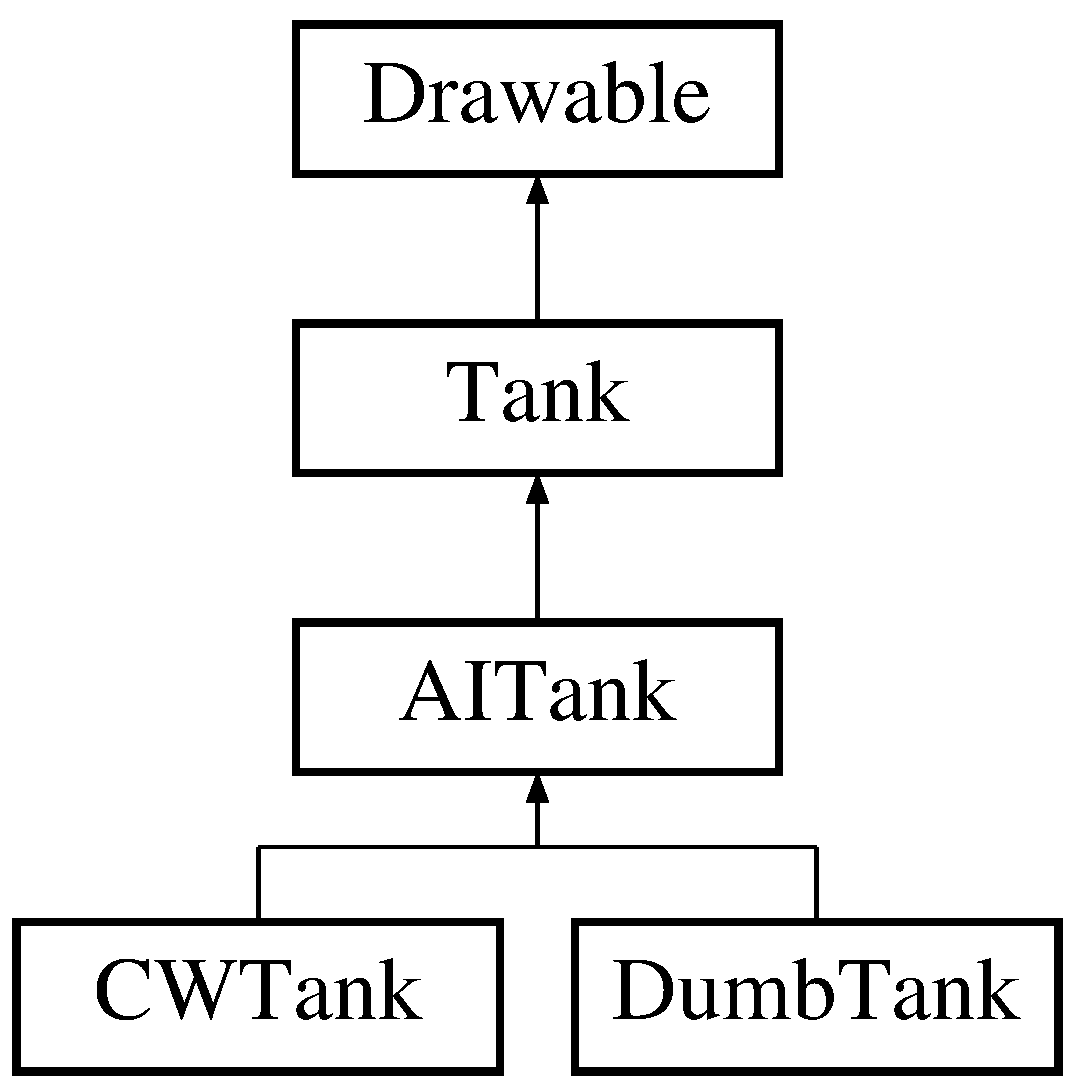
\includegraphics[height=4.000000cm]{class_a_i_tank}
\end{center}
\end{figure}
\subsection*{Public Member Functions}
\begin{DoxyCompactItemize}
\item 
\mbox{\Hypertarget{class_a_i_tank_a39ad2a5462879c2322fb737e89e60336}\label{class_a_i_tank_a39ad2a5462879c2322fb737e89e60336}} 
\mbox{\hyperlink{class_a_i_tank_a39ad2a5462879c2322fb737e89e60336}{A\+I\+Tank}} ()
\begin{DoxyCompactList}\small\item\em Empty construtor. \end{DoxyCompactList}\item 
\mbox{\Hypertarget{class_a_i_tank_ac81044895eba1a592475969c72061333}\label{class_a_i_tank_ac81044895eba1a592475969c72061333}} 
void \mbox{\hyperlink{class_a_i_tank_ac81044895eba1a592475969c72061333}{set\+Visible}} ()
\begin{DoxyCompactList}\small\item\em Make the AI tank visible to the player. \end{DoxyCompactList}\item 
\mbox{\Hypertarget{class_a_i_tank_a3c7f8e031ea59a6441c95c60c78563f0}\label{class_a_i_tank_a3c7f8e031ea59a6441c95c60c78563f0}} 
void \mbox{\hyperlink{class_a_i_tank_a3c7f8e031ea59a6441c95c60c78563f0}{set\+Invisible}} ()
\begin{DoxyCompactList}\small\item\em Make the AI tank invisible to the player. \end{DoxyCompactList}\item 
\mbox{\Hypertarget{class_a_i_tank_a1b21341fbc8cc144425742b162a536fe}\label{class_a_i_tank_a1b21341fbc8cc144425742b162a536fe}} 
bool \mbox{\hyperlink{class_a_i_tank_a1b21341fbc8cc144425742b162a536fe}{is\+Visible}} () const
\begin{DoxyCompactList}\small\item\em Is the tank visiable to the player? \end{DoxyCompactList}\item 
\mbox{\Hypertarget{class_a_i_tank_a0a4cb4af6e15d7db0cd2e3ac1ddbd236}\label{class_a_i_tank_a0a4cb4af6e15d7db0cd2e3ac1ddbd236}} 
virtual void \mbox{\hyperlink{class_a_i_tank_a0a4cb4af6e15d7db0cd2e3ac1ddbd236}{reset}} ()=0
\begin{DoxyCompactList}\small\item\em Reset any variables you need to whent he tank has been shot. \end{DoxyCompactList}\item 
\mbox{\Hypertarget{class_a_i_tank_a3d188a008b3c4f7e920bfc4d7ac8d7b9}\label{class_a_i_tank_a3d188a008b3c4f7e920bfc4d7ac8d7b9}} 
virtual void \mbox{\hyperlink{class_a_i_tank_a3d188a008b3c4f7e920bfc4d7ac8d7b9}{move}} ()=0
\begin{DoxyCompactList}\small\item\em Move the tank. \end{DoxyCompactList}\item 
\mbox{\Hypertarget{class_a_i_tank_a5d0274f97e4f2d5cc21eac90300fc67f}\label{class_a_i_tank_a5d0274f97e4f2d5cc21eac90300fc67f}} 
virtual void \mbox{\hyperlink{class_a_i_tank_a5d0274f97e4f2d5cc21eac90300fc67f}{collided}} ()=0
\begin{DoxyCompactList}\small\item\em Called by the game object when the tank has collided. \end{DoxyCompactList}\item 
virtual void \mbox{\hyperlink{class_a_i_tank_ae59c2164c71b51eeada7d2f7ef6c6238}{mark\+Target}} (\mbox{\hyperlink{class_position}{Position}} p)=0
\begin{DoxyCompactList}\small\item\em Called by the game object when a target (enemy building) comes within the tanks visible range. \end{DoxyCompactList}\item 
virtual void \mbox{\hyperlink{class_a_i_tank_a2bd0495cee5e50d3ef60b3d6c6c145d8}{mark\+Enemy}} (\mbox{\hyperlink{class_position}{Position}} p)=0
\begin{DoxyCompactList}\small\item\em Called by the game object when the enemy tank comes within the tanks visible range. \end{DoxyCompactList}\item 
virtual void \mbox{\hyperlink{class_a_i_tank_ac6d5bd1dbf2c4ccf3b6437ab17b3c5d9}{mark\+Base}} (\mbox{\hyperlink{class_position}{Position}} p)=0
\begin{DoxyCompactList}\small\item\em Called by the game object when one of you own buildings comes within the tanks visible range. \end{DoxyCompactList}\item 
virtual void \mbox{\hyperlink{class_a_i_tank_abdf630572f1bb4afcd11a711f19a7c65}{mark\+Shell}} (\mbox{\hyperlink{class_position}{Position}} p)=0
\begin{DoxyCompactList}\small\item\em Called by the game object when enemy shell comes within the tanks visible range. \end{DoxyCompactList}\item 
\mbox{\Hypertarget{class_a_i_tank_a00525c5df5a182733c2ac52031ff4e3f}\label{class_a_i_tank_a00525c5df5a182733c2ac52031ff4e3f}} 
virtual bool \mbox{\hyperlink{class_a_i_tank_a00525c5df5a182733c2ac52031ff4e3f}{is\+Firing}} ()=0
\begin{DoxyCompactList}\small\item\em Called by the game object each frame. When this function returns true (and ammo is availbe and loaded) the tank will fire a shell. \end{DoxyCompactList}\item 
\mbox{\Hypertarget{class_a_i_tank_a089bc85d0b3dcd4037f47ac35802c0c0}\label{class_a_i_tank_a089bc85d0b3dcd4037f47ac35802c0c0}} 
virtual void {\bfseries score} (int this\+Score, int enemy\+Score)=0
\end{DoxyCompactItemize}
\subsection*{Protected Attributes}
\begin{DoxyCompactItemize}
\item 
\mbox{\Hypertarget{class_a_i_tank_aa896a1b7d3d6888f2f920bf6c577e22e}\label{class_a_i_tank_aa896a1b7d3d6888f2f920bf6c577e22e}} 
bool {\bfseries visible}
\end{DoxyCompactItemize}
\subsection*{Additional Inherited Members}


\subsection{Member Function Documentation}
\mbox{\Hypertarget{class_a_i_tank_ac6d5bd1dbf2c4ccf3b6437ab17b3c5d9}\label{class_a_i_tank_ac6d5bd1dbf2c4ccf3b6437ab17b3c5d9}} 
\index{A\+I\+Tank@{A\+I\+Tank}!mark\+Base@{mark\+Base}}
\index{mark\+Base@{mark\+Base}!A\+I\+Tank@{A\+I\+Tank}}
\subsubsection{\texorpdfstring{mark\+Base()}{markBase()}}
{\footnotesize\ttfamily virtual void A\+I\+Tank\+::mark\+Base (\begin{DoxyParamCaption}\item[{\mbox{\hyperlink{class_position}{Position}}}]{p }\end{DoxyParamCaption})\hspace{0.3cm}{\ttfamily [pure virtual]}}



Called by the game object when one of you own buildings comes within the tanks visible range. 


\begin{DoxyParams}{Parameters}
{\em p} & \\
\hline
{\em \mbox{\hyperlink{class_position}{Position}}} & of the home building \\
\hline
\end{DoxyParams}


Implemented in \mbox{\hyperlink{class_c_w_tank_aa9d187d34afdf60750da9fe184f62b75}{C\+W\+Tank}}, and \mbox{\hyperlink{class_dumb_tank_ac2c8fe2a13fe009676580b33be241f59}{Dumb\+Tank}}.

\mbox{\Hypertarget{class_a_i_tank_a2bd0495cee5e50d3ef60b3d6c6c145d8}\label{class_a_i_tank_a2bd0495cee5e50d3ef60b3d6c6c145d8}} 
\index{A\+I\+Tank@{A\+I\+Tank}!mark\+Enemy@{mark\+Enemy}}
\index{mark\+Enemy@{mark\+Enemy}!A\+I\+Tank@{A\+I\+Tank}}
\subsubsection{\texorpdfstring{mark\+Enemy()}{markEnemy()}}
{\footnotesize\ttfamily virtual void A\+I\+Tank\+::mark\+Enemy (\begin{DoxyParamCaption}\item[{\mbox{\hyperlink{class_position}{Position}}}]{p }\end{DoxyParamCaption})\hspace{0.3cm}{\ttfamily [pure virtual]}}



Called by the game object when the enemy tank comes within the tanks visible range. 


\begin{DoxyParams}{Parameters}
{\em p} & \\
\hline
{\em \mbox{\hyperlink{class_position}{Position}}} & of the enemy tank \\
\hline
\end{DoxyParams}


Implemented in \mbox{\hyperlink{class_c_w_tank_ac314256fd8738022b97b0239db6955e6}{C\+W\+Tank}}, and \mbox{\hyperlink{class_dumb_tank_a6e285a834c2f65bc559c0f08133acc3e}{Dumb\+Tank}}.

\mbox{\Hypertarget{class_a_i_tank_abdf630572f1bb4afcd11a711f19a7c65}\label{class_a_i_tank_abdf630572f1bb4afcd11a711f19a7c65}} 
\index{A\+I\+Tank@{A\+I\+Tank}!mark\+Shell@{mark\+Shell}}
\index{mark\+Shell@{mark\+Shell}!A\+I\+Tank@{A\+I\+Tank}}
\subsubsection{\texorpdfstring{mark\+Shell()}{markShell()}}
{\footnotesize\ttfamily virtual void A\+I\+Tank\+::mark\+Shell (\begin{DoxyParamCaption}\item[{\mbox{\hyperlink{class_position}{Position}}}]{p }\end{DoxyParamCaption})\hspace{0.3cm}{\ttfamily [pure virtual]}}



Called by the game object when enemy shell comes within the tanks visible range. 


\begin{DoxyParams}{Parameters}
{\em p} & \\
\hline
{\em \mbox{\hyperlink{class_position}{Position}}} & of an enemy shell \\
\hline
\end{DoxyParams}


Implemented in \mbox{\hyperlink{class_c_w_tank_aacb17e0a669da6e27ab75d7df088bca7}{C\+W\+Tank}}, and \mbox{\hyperlink{class_dumb_tank_a1269c78542b1f504a388aa04fdecc4a8}{Dumb\+Tank}}.

\mbox{\Hypertarget{class_a_i_tank_ae59c2164c71b51eeada7d2f7ef6c6238}\label{class_a_i_tank_ae59c2164c71b51eeada7d2f7ef6c6238}} 
\index{A\+I\+Tank@{A\+I\+Tank}!mark\+Target@{mark\+Target}}
\index{mark\+Target@{mark\+Target}!A\+I\+Tank@{A\+I\+Tank}}
\subsubsection{\texorpdfstring{mark\+Target()}{markTarget()}}
{\footnotesize\ttfamily virtual void A\+I\+Tank\+::mark\+Target (\begin{DoxyParamCaption}\item[{\mbox{\hyperlink{class_position}{Position}}}]{p }\end{DoxyParamCaption})\hspace{0.3cm}{\ttfamily [pure virtual]}}



Called by the game object when a target (enemy building) comes within the tanks visible range. 


\begin{DoxyParams}{Parameters}
{\em p} & \\
\hline
{\em \mbox{\hyperlink{class_position}{Position}}} & of the acquired target \\
\hline
\end{DoxyParams}


Implemented in \mbox{\hyperlink{class_c_w_tank_a71b365910d43b8c41578087c9c8d8885}{C\+W\+Tank}}, and \mbox{\hyperlink{class_dumb_tank_a06dd83683ff628421d6841a8ad8f1877}{Dumb\+Tank}}.



The documentation for this class was generated from the following files\+:\begin{DoxyCompactItemize}
\item 
aitank.\+h\item 
aitank.\+cpp\end{DoxyCompactItemize}

\hypertarget{class_a_i_t_a_n_k}{}\section{A\+I\+T\+A\+NK Class Reference}
\label{class_a_i_t_a_n_k}\index{A\+I\+T\+A\+NK@{A\+I\+T\+A\+NK}}


\subsection{Detailed Description}
AI \mbox{\hyperlink{class_tank}{Tank}} 

The documentation for this class was generated from the following file\+:\begin{DoxyCompactItemize}
\item 
aitank.\+h\end{DoxyCompactItemize}

\hypertarget{class_bounding_box}{}\section{Bounding\+Box Class Reference}
\label{class_bounding_box}\index{Bounding\+Box@{Bounding\+Box}}
Inheritance diagram for Bounding\+Box\+:\begin{figure}[H]
\begin{center}
\leavevmode
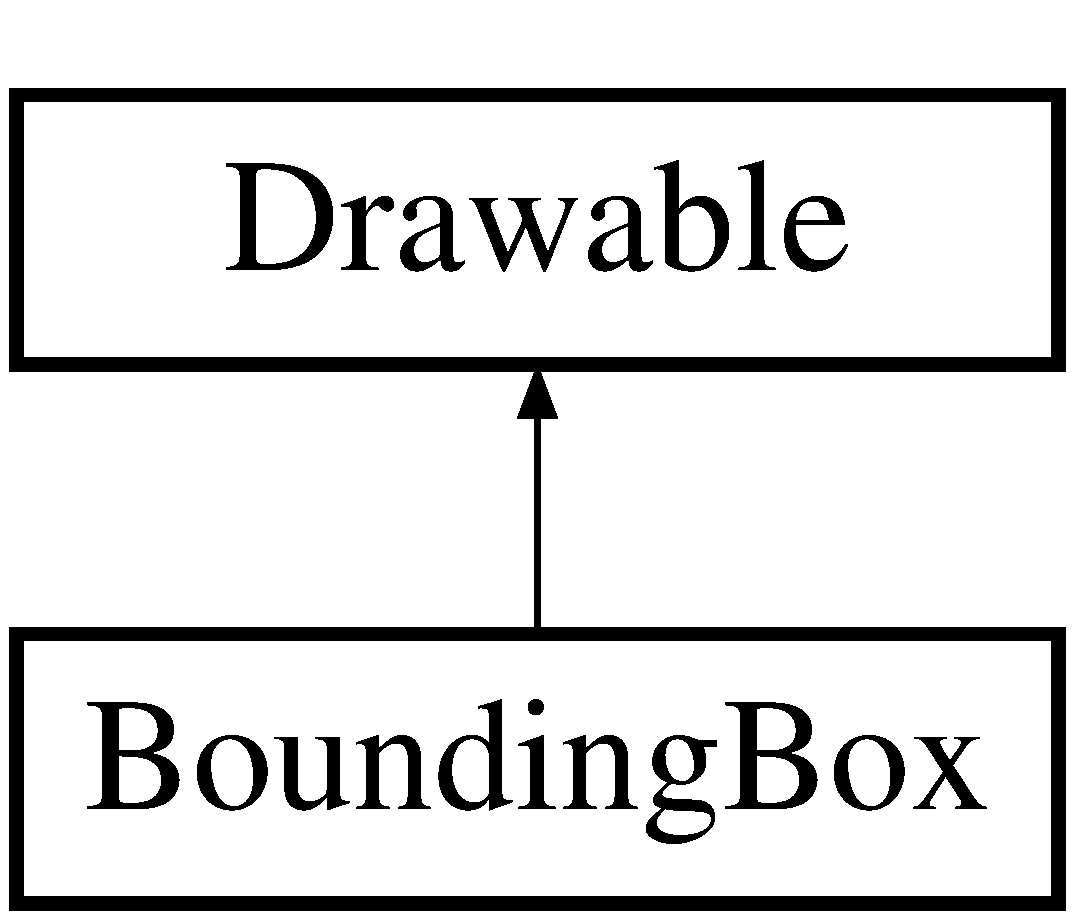
\includegraphics[height=2.000000cm]{class_bounding_box}
\end{center}
\end{figure}
\subsection*{Public Member Functions}
\begin{DoxyCompactItemize}
\item 
\mbox{\Hypertarget{class_bounding_box_a6e401c4da5839950f1f30c8b8c4d1208}\label{class_bounding_box_a6e401c4da5839950f1f30c8b8c4d1208}} 
\mbox{\hyperlink{class_bounding_box_a6e401c4da5839950f1f30c8b8c4d1208}{Bounding\+Box}} ()
\begin{DoxyCompactList}\small\item\em Empty construtor. \end{DoxyCompactList}\item 
\mbox{\Hypertarget{class_bounding_box_ae43a16b23a21e4a1e2555033839b8a87}\label{class_bounding_box_ae43a16b23a21e4a1e2555033839b8a87}} 
virtual void {\bfseries draw} (sf\+::\+Render\+Target \&target, sf\+::\+Render\+States states) const
\item 
\mbox{\Hypertarget{class_bounding_box_aff19c04b931017df2c5bb499ac251896}\label{class_bounding_box_aff19c04b931017df2c5bb499ac251896}} 
void {\bfseries set} (float xa, float ya, float xb, float yb)
\item 
\mbox{\Hypertarget{class_bounding_box_a6f709d06496c1804f0106cfd2ee8a0c8}\label{class_bounding_box_a6f709d06496c1804f0106cfd2ee8a0c8}} 
float {\bfseries get\+X1} () const
\item 
\mbox{\Hypertarget{class_bounding_box_a99cee35b530aabcc207c2a42c6ac5ba6}\label{class_bounding_box_a99cee35b530aabcc207c2a42c6ac5ba6}} 
float {\bfseries get\+Y1} () const
\item 
\mbox{\Hypertarget{class_bounding_box_a8be853a7269e34b87065ada4303f4b9d}\label{class_bounding_box_a8be853a7269e34b87065ada4303f4b9d}} 
float {\bfseries get\+X2} () const
\item 
\mbox{\Hypertarget{class_bounding_box_a52d540e2b74fe63af7671b5767cc0cec}\label{class_bounding_box_a52d540e2b74fe63af7671b5767cc0cec}} 
float {\bfseries get\+Y2} () const
\item 
\mbox{\Hypertarget{class_bounding_box_a89d92b61c3b25a6b2c05f3682e0f11f2}\label{class_bounding_box_a89d92b61c3b25a6b2c05f3682e0f11f2}} 
float {\bfseries get\+Xc} () const
\item 
\mbox{\Hypertarget{class_bounding_box_a145497b1a9064596397224e7b15702c9}\label{class_bounding_box_a145497b1a9064596397224e7b15702c9}} 
float {\bfseries get\+Yc} () const
\item 
\mbox{\Hypertarget{class_bounding_box_a2e443c907694f79293bdef5dedfd9319}\label{class_bounding_box_a2e443c907694f79293bdef5dedfd9319}} 
bool {\bfseries collision} (\mbox{\hyperlink{class_bounding_box}{Bounding\+Box}} other\+Bb) const
\item 
\mbox{\Hypertarget{class_bounding_box_a406de3f6c30f7bdc1fb0bbb840144c71}\label{class_bounding_box_a406de3f6c30f7bdc1fb0bbb840144c71}} 
bool {\bfseries line\+Collision} (float x1, float y1, float x2, float y2) const
\end{DoxyCompactItemize}


The documentation for this class was generated from the following files\+:\begin{DoxyCompactItemize}
\item 
bounding\+Box.\+h\item 
bounding\+Box.\+cpp\end{DoxyCompactItemize}

\hypertarget{class_cell_manager}{}\section{Cell\+Manager Class Reference}
\label{class_cell_manager}\index{Cell\+Manager@{Cell\+Manager}}
\subsection*{Public Member Functions}
\begin{DoxyCompactItemize}
\item 
\mbox{\hyperlink{class_cell_manager_aa0f293fc17a96f4622e5f9d3bec0928f}{Cell\+Manager}} (int x, int y, int height, int width, int row, int column)
\begin{DoxyCompactList}\small\item\em Constructor. \end{DoxyCompactList}\item 
void \mbox{\hyperlink{class_cell_manager_a5483d8656d8ef20de0b88c3fdaa44b4c}{Draw\+Cell}} (sf\+::\+Render\+Target \&target)
\item 
\mbox{\Hypertarget{class_cell_manager_a5bd4479c2fe3b57f61c365578c34aa59}\label{class_cell_manager_a5bd4479c2fe3b57f61c365578c34aa59}} 
int \mbox{\hyperlink{class_cell_manager_a5bd4479c2fe3b57f61c365578c34aa59}{getX}} ()
\begin{DoxyCompactList}\small\item\em Get the X value. \end{DoxyCompactList}\item 
\mbox{\Hypertarget{class_cell_manager_a21092ba64a338efd69139ab413451acb}\label{class_cell_manager_a21092ba64a338efd69139ab413451acb}} 
int \mbox{\hyperlink{class_cell_manager_a21092ba64a338efd69139ab413451acb}{getY}} ()
\begin{DoxyCompactList}\small\item\em Get the Y value. \end{DoxyCompactList}\item 
\mbox{\Hypertarget{class_cell_manager_a9ccf04ba5e359690d85b6a3d309f00b1}\label{class_cell_manager_a9ccf04ba5e359690d85b6a3d309f00b1}} 
void \mbox{\hyperlink{class_cell_manager_a9ccf04ba5e359690d85b6a3d309f00b1}{set\+Wall}} ()
\begin{DoxyCompactList}\small\item\em Set wall. \end{DoxyCompactList}\item 
\mbox{\Hypertarget{class_cell_manager_af8df05e6720c3a35b68ee8ace9494810}\label{class_cell_manager_af8df05e6720c3a35b68ee8ace9494810}} 
void \mbox{\hyperlink{class_cell_manager_af8df05e6720c3a35b68ee8ace9494810}{set\+Path}} ()
\begin{DoxyCompactList}\small\item\em Set the path. \end{DoxyCompactList}\item 
\mbox{\Hypertarget{class_cell_manager_ac883cd92316dab0de2970504b4485d59}\label{class_cell_manager_ac883cd92316dab0de2970504b4485d59}} 
void \mbox{\hyperlink{class_cell_manager_ac883cd92316dab0de2970504b4485d59}{set\+Goal}} ()
\begin{DoxyCompactList}\small\item\em Set the goal. \end{DoxyCompactList}\item 
\mbox{\Hypertarget{class_cell_manager_ac105b2613f3c976a86562777d254b486}\label{class_cell_manager_ac105b2613f3c976a86562777d254b486}} 
void \mbox{\hyperlink{class_cell_manager_ac105b2613f3c976a86562777d254b486}{set\+Start}} ()
\begin{DoxyCompactList}\small\item\em Set the start node. \end{DoxyCompactList}\item 
\mbox{\Hypertarget{class_cell_manager_a744dc1d4a66749a7e4f6f6489451eb2d}\label{class_cell_manager_a744dc1d4a66749a7e4f6f6489451eb2d}} 
void \mbox{\hyperlink{class_cell_manager_a744dc1d4a66749a7e4f6f6489451eb2d}{set\+Open}} ()
\begin{DoxyCompactList}\small\item\em Set open. \end{DoxyCompactList}\item 
\mbox{\Hypertarget{class_cell_manager_a177a7b719bf7d7d5befe87a08debc753}\label{class_cell_manager_a177a7b719bf7d7d5befe87a08debc753}} 
void \mbox{\hyperlink{class_cell_manager_a177a7b719bf7d7d5befe87a08debc753}{set\+Closed}} ()
\begin{DoxyCompactList}\small\item\em Set closed. \end{DoxyCompactList}\item 
void \mbox{\hyperlink{class_cell_manager_a54ad62f93aa0c271f3ebadbd45a9d941}{set\+Current}} (bool b)
\begin{DoxyCompactList}\small\item\em Set the current. \end{DoxyCompactList}\item 
int \mbox{\hyperlink{class_cell_manager_a51c6a0e10fecbe8a9e349574e3d1f69c}{lower\+Outcome}} (const \mbox{\hyperlink{class_cell_manager}{Cell\+Manager}} other) const
\begin{DoxyCompactList}\small\item\em Lower outcome? \end{DoxyCompactList}\item 
int \mbox{\hyperlink{class_cell_manager_a6243c6c1c190fb440a5b6a0630999307}{score}} (float parent\+Geo\+Score, float currentX, float currentY, int goalX, int goalY)
\begin{DoxyCompactList}\small\item\em The score of the cell. \end{DoxyCompactList}\item 
\mbox{\Hypertarget{class_cell_manager_a1deabd7112ec2f07c08180afbf7fb44d}\label{class_cell_manager_a1deabd7112ec2f07c08180afbf7fb44d}} 
\mbox{\hyperlink{class_cell_manager_a1deabd7112ec2f07c08180afbf7fb44d}{$\sim$\+Cell\+Manager}} ()
\begin{DoxyCompactList}\small\item\em Destructor. \end{DoxyCompactList}\end{DoxyCompactItemize}
\subsection*{Public Attributes}
\begin{DoxyCompactItemize}
\item 
\mbox{\Hypertarget{class_cell_manager_a6d9c7fe60c4cffeb356eb8d04c944c6d}\label{class_cell_manager_a6d9c7fe60c4cffeb356eb8d04c944c6d}} 
bool \mbox{\hyperlink{class_cell_manager_a6d9c7fe60c4cffeb356eb8d04c944c6d}{m\+\_\+b\+Current}} = true
\begin{DoxyCompactList}\small\item\em Current cell. \end{DoxyCompactList}\item 
\mbox{\Hypertarget{class_cell_manager_a4621ccf5a556eb4d32bccff37963fe81}\label{class_cell_manager_a4621ccf5a556eb4d32bccff37963fe81}} 
bool \mbox{\hyperlink{class_cell_manager_a4621ccf5a556eb4d32bccff37963fe81}{m\+\_\+b\+Not\+Right\+Path}} = false
\begin{DoxyCompactList}\small\item\em Not the right path? \end{DoxyCompactList}\item 
\mbox{\Hypertarget{class_cell_manager_ad085500cc835dff8db164ecab6ec8a35}\label{class_cell_manager_ad085500cc835dff8db164ecab6ec8a35}} 
bool \mbox{\hyperlink{class_cell_manager_ad085500cc835dff8db164ecab6ec8a35}{m\+\_\+b\+Path}} = true
\begin{DoxyCompactList}\small\item\em Path. \end{DoxyCompactList}\item 
\mbox{\Hypertarget{class_cell_manager_a1c7d4f4799002779714caf97b795114c}\label{class_cell_manager_a1c7d4f4799002779714caf97b795114c}} 
float \mbox{\hyperlink{class_cell_manager_a1c7d4f4799002779714caf97b795114c}{m\+\_\+f\+Cost}}
\begin{DoxyCompactList}\small\item\em Cost of a cell. \end{DoxyCompactList}\item 
\mbox{\Hypertarget{class_cell_manager_a4646c59c088b6b8edafb9f40088976b5}\label{class_cell_manager_a4646c59c088b6b8edafb9f40088976b5}} 
float \mbox{\hyperlink{class_cell_manager_a4646c59c088b6b8edafb9f40088976b5}{m\+\_\+f\+Dist\+Current\+To\+Start}}
\begin{DoxyCompactList}\small\item\em Distance of the current cell from the start cell. \end{DoxyCompactList}\item 
\mbox{\Hypertarget{class_cell_manager_ae515543daf0ae8d9838f8b481cd5ae05}\label{class_cell_manager_ae515543daf0ae8d9838f8b481cd5ae05}} 
float {\bfseries m\+\_\+f\+Dist\+Current\+To\+Goal}
\item 
\mbox{\Hypertarget{class_cell_manager_a6d3b28289ad1655a7447ce26bb2d4cf3}\label{class_cell_manager_a6d3b28289ad1655a7447ce26bb2d4cf3}} 
int \mbox{\hyperlink{class_cell_manager_a6d3b28289ad1655a7447ce26bb2d4cf3}{parent}}
\begin{DoxyCompactList}\small\item\em Parent cell. \end{DoxyCompactList}\item 
\mbox{\Hypertarget{class_cell_manager_a067eeb6e400cfd443b9375ec0dad0186}\label{class_cell_manager_a067eeb6e400cfd443b9375ec0dad0186}} 
int \mbox{\hyperlink{class_cell_manager_a067eeb6e400cfd443b9375ec0dad0186}{m\+\_\+i\+Row}}
\begin{DoxyCompactList}\small\item\em Row. \end{DoxyCompactList}\item 
\mbox{\Hypertarget{class_cell_manager_a694ac6bd428aab0cff7355dda80468ad}\label{class_cell_manager_a694ac6bd428aab0cff7355dda80468ad}} 
int \mbox{\hyperlink{class_cell_manager_a694ac6bd428aab0cff7355dda80468ad}{m\+\_\+i\+Column}}
\begin{DoxyCompactList}\small\item\em Column. \end{DoxyCompactList}\end{DoxyCompactItemize}


\subsection{Constructor \& Destructor Documentation}
\mbox{\Hypertarget{class_cell_manager_aa0f293fc17a96f4622e5f9d3bec0928f}\label{class_cell_manager_aa0f293fc17a96f4622e5f9d3bec0928f}} 
\index{Cell\+Manager@{Cell\+Manager}!Cell\+Manager@{Cell\+Manager}}
\index{Cell\+Manager@{Cell\+Manager}!Cell\+Manager@{Cell\+Manager}}
\subsubsection{\texorpdfstring{Cell\+Manager()}{CellManager()}}
{\footnotesize\ttfamily Cell\+Manager\+::\+Cell\+Manager (\begin{DoxyParamCaption}\item[{int}]{x,  }\item[{int}]{y,  }\item[{int}]{height,  }\item[{int}]{width,  }\item[{int}]{row,  }\item[{int}]{column }\end{DoxyParamCaption})}



Constructor. 


\begin{DoxyParams}{Parameters}
{\em x} & \\
\hline
{\em x} & position \\
\hline
{\em y} & \\
\hline
{\em y} & position \\
\hline
{\em height} & \\
\hline
{\em height} & of the cell \\
\hline
{\em width} & \\
\hline
{\em width} & of the cell \\
\hline
{\em row} & \\
\hline
{\em rows} & \\
\hline
{\em column} & \\
\hline
{\em columns} & \\
\hline
\end{DoxyParams}


\subsection{Member Function Documentation}
\mbox{\Hypertarget{class_cell_manager_a5483d8656d8ef20de0b88c3fdaa44b4c}\label{class_cell_manager_a5483d8656d8ef20de0b88c3fdaa44b4c}} 
\index{Cell\+Manager@{Cell\+Manager}!Draw\+Cell@{Draw\+Cell}}
\index{Draw\+Cell@{Draw\+Cell}!Cell\+Manager@{Cell\+Manager}}
\subsubsection{\texorpdfstring{Draw\+Cell()}{DrawCell()}}
{\footnotesize\ttfamily void Cell\+Manager\+::\+Draw\+Cell (\begin{DoxyParamCaption}\item[{sf\+::\+Render\+Target \&}]{target }\end{DoxyParamCaption})}


\begin{DoxyParams}{Parameters}
{\em target} & \\
\hline
{\em target} & to draw a cell to. \\
\hline
\end{DoxyParams}
\mbox{\Hypertarget{class_cell_manager_a51c6a0e10fecbe8a9e349574e3d1f69c}\label{class_cell_manager_a51c6a0e10fecbe8a9e349574e3d1f69c}} 
\index{Cell\+Manager@{Cell\+Manager}!lower\+Outcome@{lower\+Outcome}}
\index{lower\+Outcome@{lower\+Outcome}!Cell\+Manager@{Cell\+Manager}}
\subsubsection{\texorpdfstring{lower\+Outcome()}{lowerOutcome()}}
{\footnotesize\ttfamily int Cell\+Manager\+::lower\+Outcome (\begin{DoxyParamCaption}\item[{const \mbox{\hyperlink{class_cell_manager}{Cell\+Manager}}}]{other }\end{DoxyParamCaption}) const}



Lower outcome? 


\begin{DoxyParams}{Parameters}
{\em other} & \\
\hline
{\em the} & other cell \\
\hline
\end{DoxyParams}
\mbox{\Hypertarget{class_cell_manager_a6243c6c1c190fb440a5b6a0630999307}\label{class_cell_manager_a6243c6c1c190fb440a5b6a0630999307}} 
\index{Cell\+Manager@{Cell\+Manager}!score@{score}}
\index{score@{score}!Cell\+Manager@{Cell\+Manager}}
\subsubsection{\texorpdfstring{score()}{score()}}
{\footnotesize\ttfamily int Cell\+Manager\+::score (\begin{DoxyParamCaption}\item[{float}]{parent\+Geo\+Score,  }\item[{float}]{currentX,  }\item[{float}]{currentY,  }\item[{int}]{goalX,  }\item[{int}]{goalY }\end{DoxyParamCaption})}



The score of the cell. 


\begin{DoxyParams}{Parameters}
{\em parent\+Geo\+Score} & \\
\hline
{\em parent} & cell\textquotesingle{}s geographical score \\
\hline
{\em currentX} & \\
\hline
{\em current} & x position \\
\hline
{\em currentY} & \\
\hline
{\em current} & y position \\
\hline
{\em goalX} & \\
\hline
{\em goal} & x position \\
\hline
{\em goalY} & \\
\hline
{\em goal} & y position \\
\hline
\end{DoxyParams}
\mbox{\Hypertarget{class_cell_manager_a54ad62f93aa0c271f3ebadbd45a9d941}\label{class_cell_manager_a54ad62f93aa0c271f3ebadbd45a9d941}} 
\index{Cell\+Manager@{Cell\+Manager}!set\+Current@{set\+Current}}
\index{set\+Current@{set\+Current}!Cell\+Manager@{Cell\+Manager}}
\subsubsection{\texorpdfstring{set\+Current()}{setCurrent()}}
{\footnotesize\ttfamily void Cell\+Manager\+::set\+Current (\begin{DoxyParamCaption}\item[{bool}]{b }\end{DoxyParamCaption})}



Set the current. 


\begin{DoxyParams}{Parameters}
{\em b} & \\
\hline
{\em is} & it current \\
\hline
\end{DoxyParams}


The documentation for this class was generated from the following files\+:\begin{DoxyCompactItemize}
\item 
Cell\+Manager.\+h\item 
Cell\+Manager.\+cpp\end{DoxyCompactItemize}

\hypertarget{class_cell_map}{}\section{Cell\+Map Class Reference}
\label{class_cell_map}\index{Cell\+Map@{Cell\+Map}}
\subsection*{Public Member Functions}
\begin{DoxyCompactItemize}
\item 
\mbox{\Hypertarget{class_cell_map_af5e47ca959f63f4678a4346f773030f7}\label{class_cell_map_af5e47ca959f63f4678a4346f773030f7}} 
\mbox{\hyperlink{class_cell_map_af5e47ca959f63f4678a4346f773030f7}{Cell\+Map}} ()
\begin{DoxyCompactList}\small\item\em Constructor. \end{DoxyCompactList}\item 
void \mbox{\hyperlink{class_cell_map_a64c4abb5efb6540e34e7bb73bdb12e76}{Draw\+Map}} (sf\+::\+Render\+Target \&target)
\begin{DoxyCompactList}\small\item\em Draw the map. \end{DoxyCompactList}\item 
void \mbox{\hyperlink{class_cell_map_a0532f2df278250c570914b4c3c8c6b5f}{not\+Path}} (sf\+::\+Vector2f pos)
\begin{DoxyCompactList}\small\item\em Not the path. \end{DoxyCompactList}\item 
void \mbox{\hyperlink{class_cell_map_a639a7552b9d5ac42f8d652db4852568d}{set\+Path}} (sf\+::\+Vector2f pos)
\begin{DoxyCompactList}\small\item\em Set the path. \end{DoxyCompactList}\item 
std\+::vector$<$ \mbox{\hyperlink{class_cell_manager}{Cell\+Manager}} $\ast$ $>$ \mbox{\hyperlink{class_cell_map_a3e63b51e165eb896c7e1900efff13245}{get\+Cell\+Neighbours}} (\mbox{\hyperlink{class_cell_manager}{Cell\+Manager}} $\ast$cell)
\begin{DoxyCompactList}\small\item\em Vector containing the current cells neighbours. \end{DoxyCompactList}\item 
bool \mbox{\hyperlink{class_cell_map_ac3abe891a8076fd0f9d134de4f1d55b4}{A\+Star}} (std\+::list$<$ \mbox{\hyperlink{class_cell_manager}{Cell\+Manager}} $>$ \&path, \mbox{\hyperlink{class_cell_manager}{Cell\+Manager}} start, \mbox{\hyperlink{class_cell_manager}{Cell\+Manager}} goal)
\begin{DoxyCompactList}\small\item\em A$\ast$ algorithm. \end{DoxyCompactList}\item 
std\+::list$<$ \mbox{\hyperlink{class_cell_manager}{Cell\+Manager}} $>$ \mbox{\hyperlink{class_cell_map_a38deb8b7767412f9d169d902614f954b}{construct\+\_\+path}} (std\+::list$<$ \mbox{\hyperlink{class_cell_manager}{Cell\+Manager}} $>$ \&path, std\+::list$<$ \mbox{\hyperlink{class_cell_manager}{Cell\+Manager}} $>$ \&closed, \mbox{\hyperlink{class_cell_manager}{Cell\+Manager}} $\ast$cell)
\begin{DoxyCompactList}\small\item\em Constuct a path. \end{DoxyCompactList}\item 
\mbox{\Hypertarget{class_cell_map_a6819c9a8c9b4032eb7fbc03d2b84f512}\label{class_cell_map_a6819c9a8c9b4032eb7fbc03d2b84f512}} 
\mbox{\hyperlink{class_cell_map_a6819c9a8c9b4032eb7fbc03d2b84f512}{$\sim$\+Cell\+Map}} ()
\begin{DoxyCompactList}\small\item\em Destructor. \end{DoxyCompactList}\end{DoxyCompactItemize}
\subsection*{Public Attributes}
\begin{DoxyCompactItemize}
\item 
\mbox{\Hypertarget{class_cell_map_ae662e21dea4d8b98350a7af1d5261836}\label{class_cell_map_ae662e21dea4d8b98350a7af1d5261836}} 
\mbox{\hyperlink{class_cell_manager}{Cell\+Manager}} $\ast$ \mbox{\hyperlink{class_cell_map_ae662e21dea4d8b98350a7af1d5261836}{map\+Array}} \mbox{[}16\mbox{]}\mbox{[}22\mbox{]}
\begin{DoxyCompactList}\small\item\em The map array, the size of it reflects the rows and columns. \end{DoxyCompactList}\end{DoxyCompactItemize}
\subsection*{Static Public Attributes}
\begin{DoxyCompactItemize}
\item 
\mbox{\Hypertarget{class_cell_map_a89b555d5fcee4435e179f276e9a7380d}\label{class_cell_map_a89b555d5fcee4435e179f276e9a7380d}} 
static const unsigned \mbox{\hyperlink{class_cell_map_a89b555d5fcee4435e179f276e9a7380d}{cells}} = m\+\_\+ki\+Rows $\ast$ m\+\_\+ki\+Columns
\begin{DoxyCompactList}\small\item\em Cells in map. \end{DoxyCompactList}\end{DoxyCompactItemize}


\subsection{Member Function Documentation}
\mbox{\Hypertarget{class_cell_map_ac3abe891a8076fd0f9d134de4f1d55b4}\label{class_cell_map_ac3abe891a8076fd0f9d134de4f1d55b4}} 
\index{Cell\+Map@{Cell\+Map}!A\+Star@{A\+Star}}
\index{A\+Star@{A\+Star}!Cell\+Map@{Cell\+Map}}
\subsubsection{\texorpdfstring{A\+Star()}{AStar()}}
{\footnotesize\ttfamily bool Cell\+Map\+::\+A\+Star (\begin{DoxyParamCaption}\item[{std\+::list$<$ \mbox{\hyperlink{class_cell_manager}{Cell\+Manager}} $>$ \&}]{path,  }\item[{\mbox{\hyperlink{class_cell_manager}{Cell\+Manager}}}]{start,  }\item[{\mbox{\hyperlink{class_cell_manager}{Cell\+Manager}}}]{goal }\end{DoxyParamCaption})}



A$\ast$ algorithm. 


\begin{DoxyParams}{Parameters}
{\em path} & \\
\hline
{\em The} & path list \\
\hline
{\em start} & \\
\hline
{\em Starting} & cell \\
\hline
{\em goal} & \\
\hline
{\em End} & cell \\
\hline
\end{DoxyParams}
\mbox{\Hypertarget{class_cell_map_a38deb8b7767412f9d169d902614f954b}\label{class_cell_map_a38deb8b7767412f9d169d902614f954b}} 
\index{Cell\+Map@{Cell\+Map}!construct\+\_\+path@{construct\+\_\+path}}
\index{construct\+\_\+path@{construct\+\_\+path}!Cell\+Map@{Cell\+Map}}
\subsubsection{\texorpdfstring{construct\+\_\+path()}{construct\_path()}}
{\footnotesize\ttfamily std\+::list$<$ \mbox{\hyperlink{class_cell_manager}{Cell\+Manager}} $>$ Cell\+Map\+::construct\+\_\+path (\begin{DoxyParamCaption}\item[{std\+::list$<$ \mbox{\hyperlink{class_cell_manager}{Cell\+Manager}} $>$ \&}]{path,  }\item[{std\+::list$<$ \mbox{\hyperlink{class_cell_manager}{Cell\+Manager}} $>$ \&}]{closed,  }\item[{\mbox{\hyperlink{class_cell_manager}{Cell\+Manager}} $\ast$}]{cell }\end{DoxyParamCaption})}



Constuct a path. 


\begin{DoxyParams}{Parameters}
{\em path} & \\
\hline
{\em The} & path list \\
\hline
{\em closed} & \\
\hline
{\em Closed} & List \\
\hline
{\em cell} & \\
\hline
{\em A} & cell \\
\hline
\end{DoxyParams}
\mbox{\Hypertarget{class_cell_map_a64c4abb5efb6540e34e7bb73bdb12e76}\label{class_cell_map_a64c4abb5efb6540e34e7bb73bdb12e76}} 
\index{Cell\+Map@{Cell\+Map}!Draw\+Map@{Draw\+Map}}
\index{Draw\+Map@{Draw\+Map}!Cell\+Map@{Cell\+Map}}
\subsubsection{\texorpdfstring{Draw\+Map()}{DrawMap()}}
{\footnotesize\ttfamily void Cell\+Map\+::\+Draw\+Map (\begin{DoxyParamCaption}\item[{sf\+::\+Render\+Target \&}]{target }\end{DoxyParamCaption})}



Draw the map. 


\begin{DoxyParams}{Parameters}
{\em target} & \\
\hline
{\em target} & to draw the cell to \\
\hline
\end{DoxyParams}
\mbox{\Hypertarget{class_cell_map_a3e63b51e165eb896c7e1900efff13245}\label{class_cell_map_a3e63b51e165eb896c7e1900efff13245}} 
\index{Cell\+Map@{Cell\+Map}!get\+Cell\+Neighbours@{get\+Cell\+Neighbours}}
\index{get\+Cell\+Neighbours@{get\+Cell\+Neighbours}!Cell\+Map@{Cell\+Map}}
\subsubsection{\texorpdfstring{get\+Cell\+Neighbours()}{getCellNeighbours()}}
{\footnotesize\ttfamily std\+::vector$<$ \mbox{\hyperlink{class_cell_manager}{Cell\+Manager}} $\ast$ $>$ Cell\+Map\+::get\+Cell\+Neighbours (\begin{DoxyParamCaption}\item[{\mbox{\hyperlink{class_cell_manager}{Cell\+Manager}} $\ast$}]{cell }\end{DoxyParamCaption})}



Vector containing the current cells neighbours. 


\begin{DoxyParams}{Parameters}
{\em cell} & \\
\hline
{\em A} & cell. \\
\hline
\end{DoxyParams}
\mbox{\Hypertarget{class_cell_map_a0532f2df278250c570914b4c3c8c6b5f}\label{class_cell_map_a0532f2df278250c570914b4c3c8c6b5f}} 
\index{Cell\+Map@{Cell\+Map}!not\+Path@{not\+Path}}
\index{not\+Path@{not\+Path}!Cell\+Map@{Cell\+Map}}
\subsubsection{\texorpdfstring{not\+Path()}{notPath()}}
{\footnotesize\ttfamily void Cell\+Map\+::not\+Path (\begin{DoxyParamCaption}\item[{sf\+::\+Vector2f}]{pos }\end{DoxyParamCaption})}



Not the path. 


\begin{DoxyParams}{Parameters}
{\em pos} & \\
\hline
{\em position} & \\
\hline
\end{DoxyParams}
\mbox{\Hypertarget{class_cell_map_a639a7552b9d5ac42f8d652db4852568d}\label{class_cell_map_a639a7552b9d5ac42f8d652db4852568d}} 
\index{Cell\+Map@{Cell\+Map}!set\+Path@{set\+Path}}
\index{set\+Path@{set\+Path}!Cell\+Map@{Cell\+Map}}
\subsubsection{\texorpdfstring{set\+Path()}{setPath()}}
{\footnotesize\ttfamily void Cell\+Map\+::set\+Path (\begin{DoxyParamCaption}\item[{sf\+::\+Vector2f}]{pos }\end{DoxyParamCaption})}



Set the path. 


\begin{DoxyParams}{Parameters}
{\em pos} & \\
\hline
{\em position} & \\
\hline
\end{DoxyParams}


The documentation for this class was generated from the following files\+:\begin{DoxyCompactItemize}
\item 
Cell\+Map.\+h\item 
Cell\+Map.\+cpp\end{DoxyCompactItemize}

\hypertarget{class_c_w_tank}{}\section{C\+W\+Tank Class Reference}
\label{class_c_w_tank}\index{C\+W\+Tank@{C\+W\+Tank}}
Inheritance diagram for C\+W\+Tank\+:\begin{figure}[H]
\begin{center}
\leavevmode
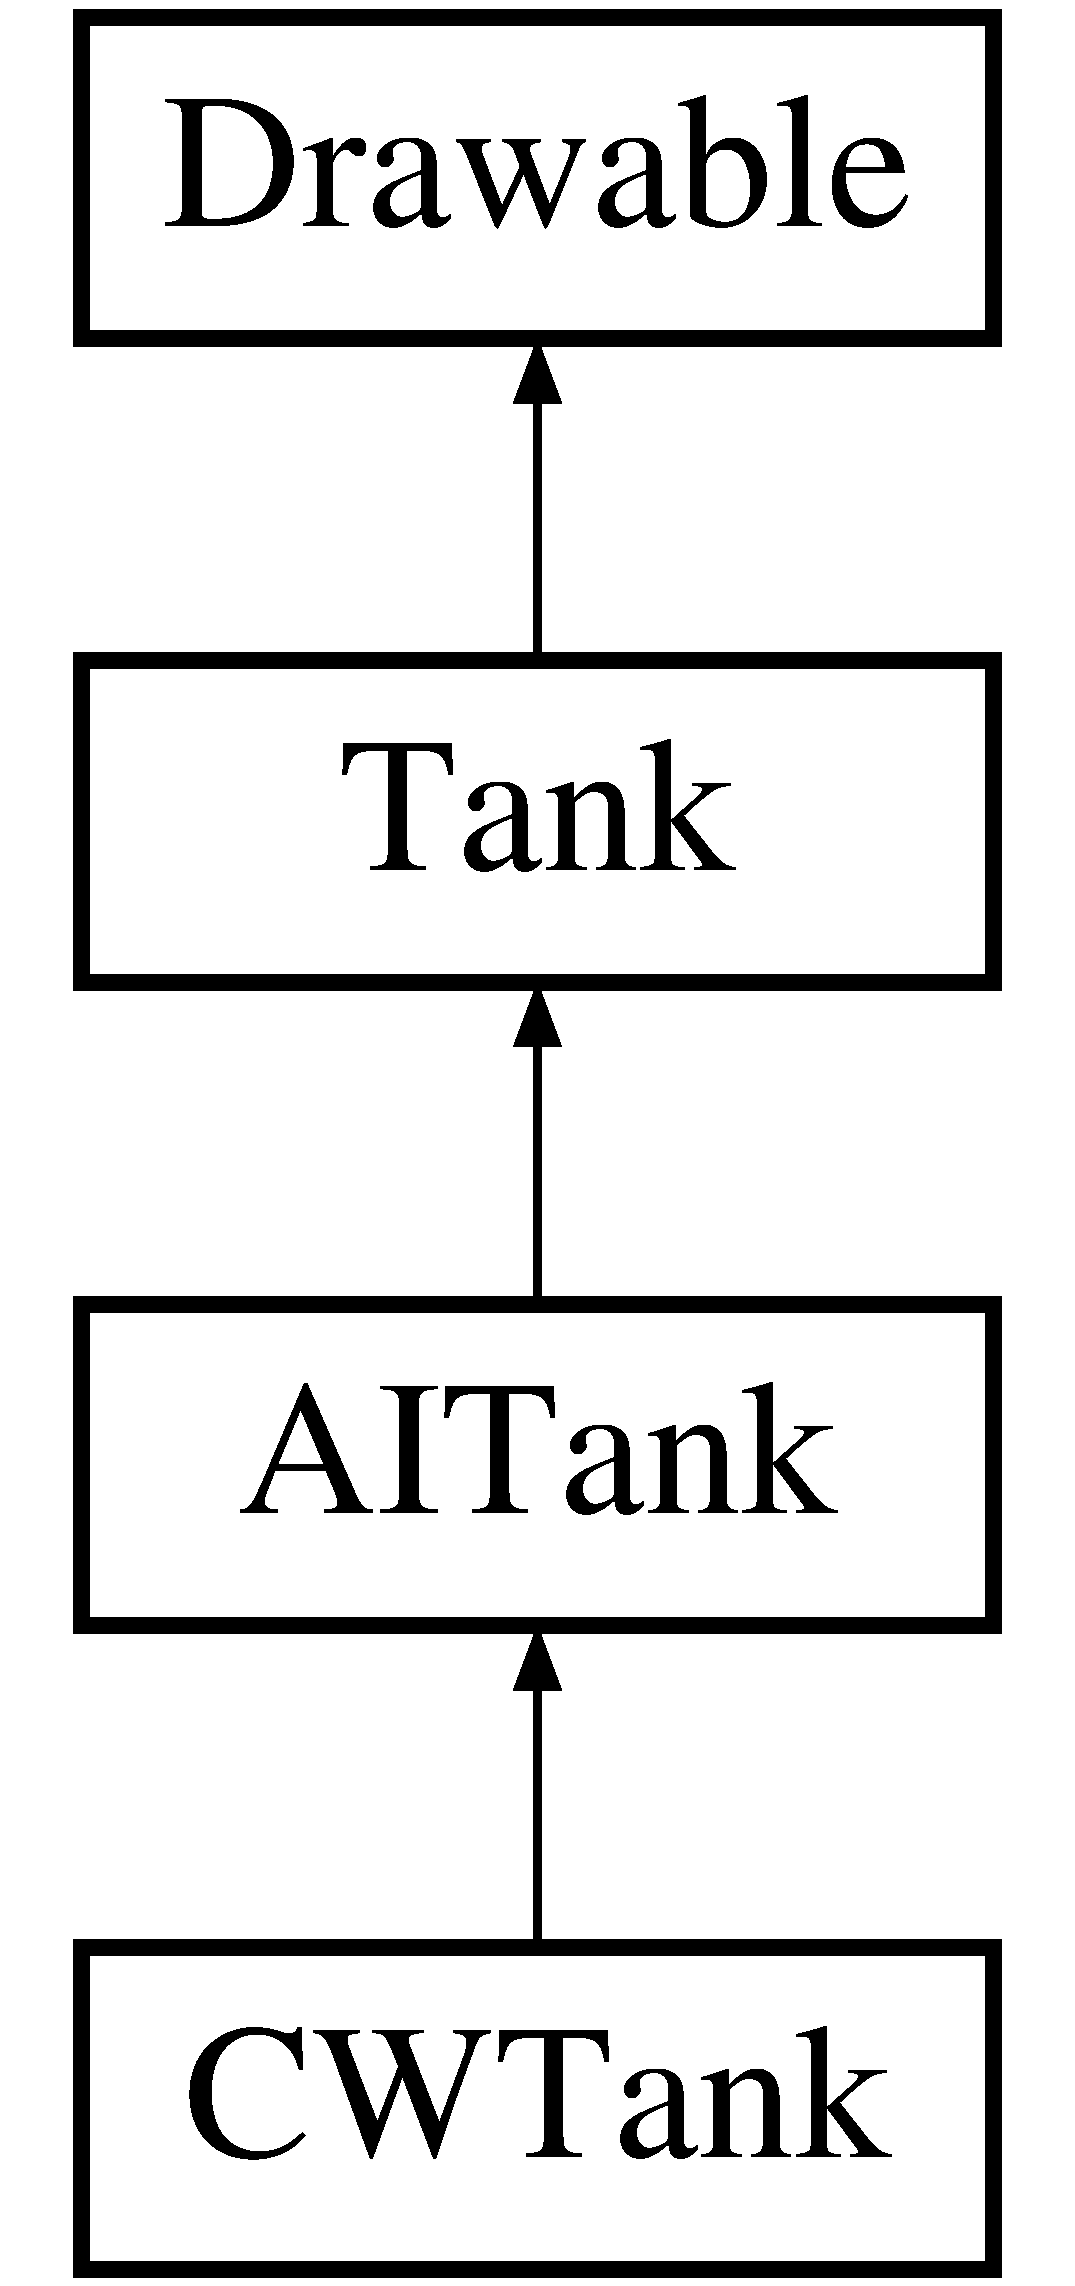
\includegraphics[height=4.000000cm]{class_c_w_tank}
\end{center}
\end{figure}
\subsection*{Public Member Functions}
\begin{DoxyCompactItemize}
\item 
\mbox{\Hypertarget{class_c_w_tank_a1bcbbdd9bac59a8ee2242ab45ab1ad2b}\label{class_c_w_tank_a1bcbbdd9bac59a8ee2242ab45ab1ad2b}} 
\mbox{\hyperlink{class_c_w_tank_a1bcbbdd9bac59a8ee2242ab45ab1ad2b}{C\+W\+Tank}} ()
\begin{DoxyCompactList}\small\item\em Constructor. \end{DoxyCompactList}\item 
\mbox{\Hypertarget{class_c_w_tank_a04b5e0c63fef1e451c1bc724d56f882b}\label{class_c_w_tank_a04b5e0c63fef1e451c1bc724d56f882b}} 
\mbox{\hyperlink{class_c_w_tank_a04b5e0c63fef1e451c1bc724d56f882b}{$\sim$\+C\+W\+Tank}} ()
\begin{DoxyCompactList}\small\item\em Destructor. \end{DoxyCompactList}\item 
\mbox{\Hypertarget{class_c_w_tank_a9b4868441133922d291e7e869ccba78a}\label{class_c_w_tank_a9b4868441133922d291e7e869ccba78a}} 
void \mbox{\hyperlink{class_c_w_tank_a9b4868441133922d291e7e869ccba78a}{move}} ()
\begin{DoxyCompactList}\small\item\em Move the tank. \end{DoxyCompactList}\item 
\mbox{\Hypertarget{class_c_w_tank_a8461e4aa3726689dd9e515ee68001804}\label{class_c_w_tank_a8461e4aa3726689dd9e515ee68001804}} 
void \mbox{\hyperlink{class_c_w_tank_a8461e4aa3726689dd9e515ee68001804}{reset}} ()
\begin{DoxyCompactList}\small\item\em Reset the tank. \end{DoxyCompactList}\item 
\mbox{\Hypertarget{class_c_w_tank_aeb13b5ea6112827346bbf4ea1cb9076b}\label{class_c_w_tank_aeb13b5ea6112827346bbf4ea1cb9076b}} 
void \mbox{\hyperlink{class_c_w_tank_aeb13b5ea6112827346bbf4ea1cb9076b}{collided}} ()
\begin{DoxyCompactList}\small\item\em Has the tank collided with anything. \end{DoxyCompactList}\item 
\mbox{\Hypertarget{class_c_w_tank_af70ef410d32daaf8e90a56a854cf6b4c}\label{class_c_w_tank_af70ef410d32daaf8e90a56a854cf6b4c}} 
void \mbox{\hyperlink{class_c_w_tank_af70ef410d32daaf8e90a56a854cf6b4c}{turret\+Machine}} ()
\begin{DoxyCompactList}\small\item\em Turret state machine. \end{DoxyCompactList}\item 
\mbox{\Hypertarget{class_c_w_tank_a2eb7fe91d1c71db4af5dff3329c5d074}\label{class_c_w_tank_a2eb7fe91d1c71db4af5dff3329c5d074}} 
void \mbox{\hyperlink{class_c_w_tank_a2eb7fe91d1c71db4af5dff3329c5d074}{move\+Machine}} ()
\begin{DoxyCompactList}\small\item\em Movement state machine. \end{DoxyCompactList}\item 
\mbox{\Hypertarget{class_c_w_tank_a6c8ced110cb42af2685904db261f1b0b}\label{class_c_w_tank_a6c8ced110cb42af2685904db261f1b0b}} 
void \mbox{\hyperlink{class_c_w_tank_a6c8ced110cb42af2685904db261f1b0b}{aim\+Machine}} ()
\begin{DoxyCompactList}\small\item\em Aiming state machine. \end{DoxyCompactList}\item 
\mbox{\Hypertarget{class_c_w_tank_a424ee36d839a9381c1b36cddacffcc46}\label{class_c_w_tank_a424ee36d839a9381c1b36cddacffcc46}} 
void \mbox{\hyperlink{class_c_w_tank_a424ee36d839a9381c1b36cddacffcc46}{nav\+Machine}} ()
\begin{DoxyCompactList}\small\item\em Navigation state machine. \end{DoxyCompactList}\item 
\mbox{\Hypertarget{class_c_w_tank_a71b365910d43b8c41578087c9c8d8885}\label{class_c_w_tank_a71b365910d43b8c41578087c9c8d8885}} 
void \mbox{\hyperlink{class_c_w_tank_a71b365910d43b8c41578087c9c8d8885}{mark\+Target}} (\mbox{\hyperlink{class_position}{Position}} p)
\begin{DoxyCompactList}\small\item\em Mark a target. \end{DoxyCompactList}\item 
\mbox{\Hypertarget{class_c_w_tank_ac314256fd8738022b97b0239db6955e6}\label{class_c_w_tank_ac314256fd8738022b97b0239db6955e6}} 
void \mbox{\hyperlink{class_c_w_tank_ac314256fd8738022b97b0239db6955e6}{mark\+Enemy}} (\mbox{\hyperlink{class_position}{Position}} p)
\begin{DoxyCompactList}\small\item\em Mark an enemy. \end{DoxyCompactList}\item 
\mbox{\Hypertarget{class_c_w_tank_aa9d187d34afdf60750da9fe184f62b75}\label{class_c_w_tank_aa9d187d34afdf60750da9fe184f62b75}} 
void \mbox{\hyperlink{class_c_w_tank_aa9d187d34afdf60750da9fe184f62b75}{mark\+Base}} (\mbox{\hyperlink{class_position}{Position}} p)
\begin{DoxyCompactList}\small\item\em Mark a base. \end{DoxyCompactList}\item 
\mbox{\Hypertarget{class_c_w_tank_aacb17e0a669da6e27ab75d7df088bca7}\label{class_c_w_tank_aacb17e0a669da6e27ab75d7df088bca7}} 
void \mbox{\hyperlink{class_c_w_tank_aacb17e0a669da6e27ab75d7df088bca7}{mark\+Shell}} (\mbox{\hyperlink{class_position}{Position}} p)
\begin{DoxyCompactList}\small\item\em Mark a shell. \end{DoxyCompactList}\item 
\mbox{\Hypertarget{class_c_w_tank_ad03d72ab86ab812ea72c786921370d8b}\label{class_c_w_tank_ad03d72ab86ab812ea72c786921370d8b}} 
bool \mbox{\hyperlink{class_c_w_tank_ad03d72ab86ab812ea72c786921370d8b}{is\+Firing}} ()
\begin{DoxyCompactList}\small\item\em Is the tank firing? \end{DoxyCompactList}\item 
\mbox{\Hypertarget{class_c_w_tank_abb42d292824aca3b25e8868c9fe43302}\label{class_c_w_tank_abb42d292824aca3b25e8868c9fe43302}} 
void \mbox{\hyperlink{class_c_w_tank_abb42d292824aca3b25e8868c9fe43302}{score}} (int this\+Score, int enemy\+Score)
\begin{DoxyCompactList}\small\item\em Score. \end{DoxyCompactList}\item 
\mbox{\Hypertarget{class_c_w_tank_a17113de02508affb4fbe15746ac977ac}\label{class_c_w_tank_a17113de02508affb4fbe15746ac977ac}} 
void \mbox{\hyperlink{class_c_w_tank_a17113de02508affb4fbe15746ac977ac}{Draw\+Node}} (sf\+::\+Render\+Target \&target)
\begin{DoxyCompactList}\small\item\em Draw the cell. \end{DoxyCompactList}\item 
\mbox{\Hypertarget{class_c_w_tank_a37dd45ebdba39debcd9d1bc44e2ca992}\label{class_c_w_tank_a37dd45ebdba39debcd9d1bc44e2ca992}} 
void \mbox{\hyperlink{class_c_w_tank_a37dd45ebdba39debcd9d1bc44e2ca992}{set\+Current\+Cell}} ()
\begin{DoxyCompactList}\small\item\em Set the current cell. \end{DoxyCompactList}\item 
\mbox{\Hypertarget{class_c_w_tank_a4e1c5106a09807ad25295b696c0e7525}\label{class_c_w_tank_a4e1c5106a09807ad25295b696c0e7525}} 
sf\+::\+Rectangle\+Shape \mbox{\hyperlink{class_c_w_tank_a4e1c5106a09807ad25295b696c0e7525}{draw\+Range}} () const
\begin{DoxyCompactList}\small\item\em Draw the range. \end{DoxyCompactList}\end{DoxyCompactItemize}
\subsection*{Public Attributes}
\begin{DoxyCompactItemize}
\item 
\mbox{\Hypertarget{class_c_w_tank_ac18fc7979fc397fa3ab2cc64f90d2bb6}\label{class_c_w_tank_ac18fc7979fc397fa3ab2cc64f90d2bb6}} 
int \mbox{\hyperlink{class_c_w_tank_ac18fc7979fc397fa3ab2cc64f90d2bb6}{m\+\_\+i\+Buildings\+Remain}} = 10
\begin{DoxyCompactList}\small\item\em How many buildings remain. \end{DoxyCompactList}\item 
\mbox{\Hypertarget{class_c_w_tank_ad9b30cb1f9284dbf89821f5d4084dd70}\label{class_c_w_tank_ad9b30cb1f9284dbf89821f5d4084dd70}} 
\mbox{\hyperlink{class_cell_manager}{Cell\+Manager}} $\ast$ \mbox{\hyperlink{class_c_w_tank_ad9b30cb1f9284dbf89821f5d4084dd70}{cell}}
\begin{DoxyCompactList}\small\item\em Cell. \end{DoxyCompactList}\item 
\mbox{\Hypertarget{class_c_w_tank_ac0c2722b26c2138d539114f60802d707}\label{class_c_w_tank_ac0c2722b26c2138d539114f60802d707}} 
\mbox{\hyperlink{class_cell_map}{Cell\+Map}} $\ast$ \mbox{\hyperlink{class_c_w_tank_ac0c2722b26c2138d539114f60802d707}{map}}
\begin{DoxyCompactList}\small\item\em Map. \end{DoxyCompactList}\end{DoxyCompactItemize}
\subsection*{Additional Inherited Members}


The documentation for this class was generated from the following files\+:\begin{DoxyCompactItemize}
\item 
C\+W\+Tank.\+h\item 
C\+W\+Tank.\+cpp\end{DoxyCompactItemize}

\hypertarget{class_dumb_tank}{}\section{Dumb\+Tank Class Reference}
\label{class_dumb_tank}\index{Dumb\+Tank@{Dumb\+Tank}}
Inheritance diagram for Dumb\+Tank\+:\begin{figure}[H]
\begin{center}
\leavevmode
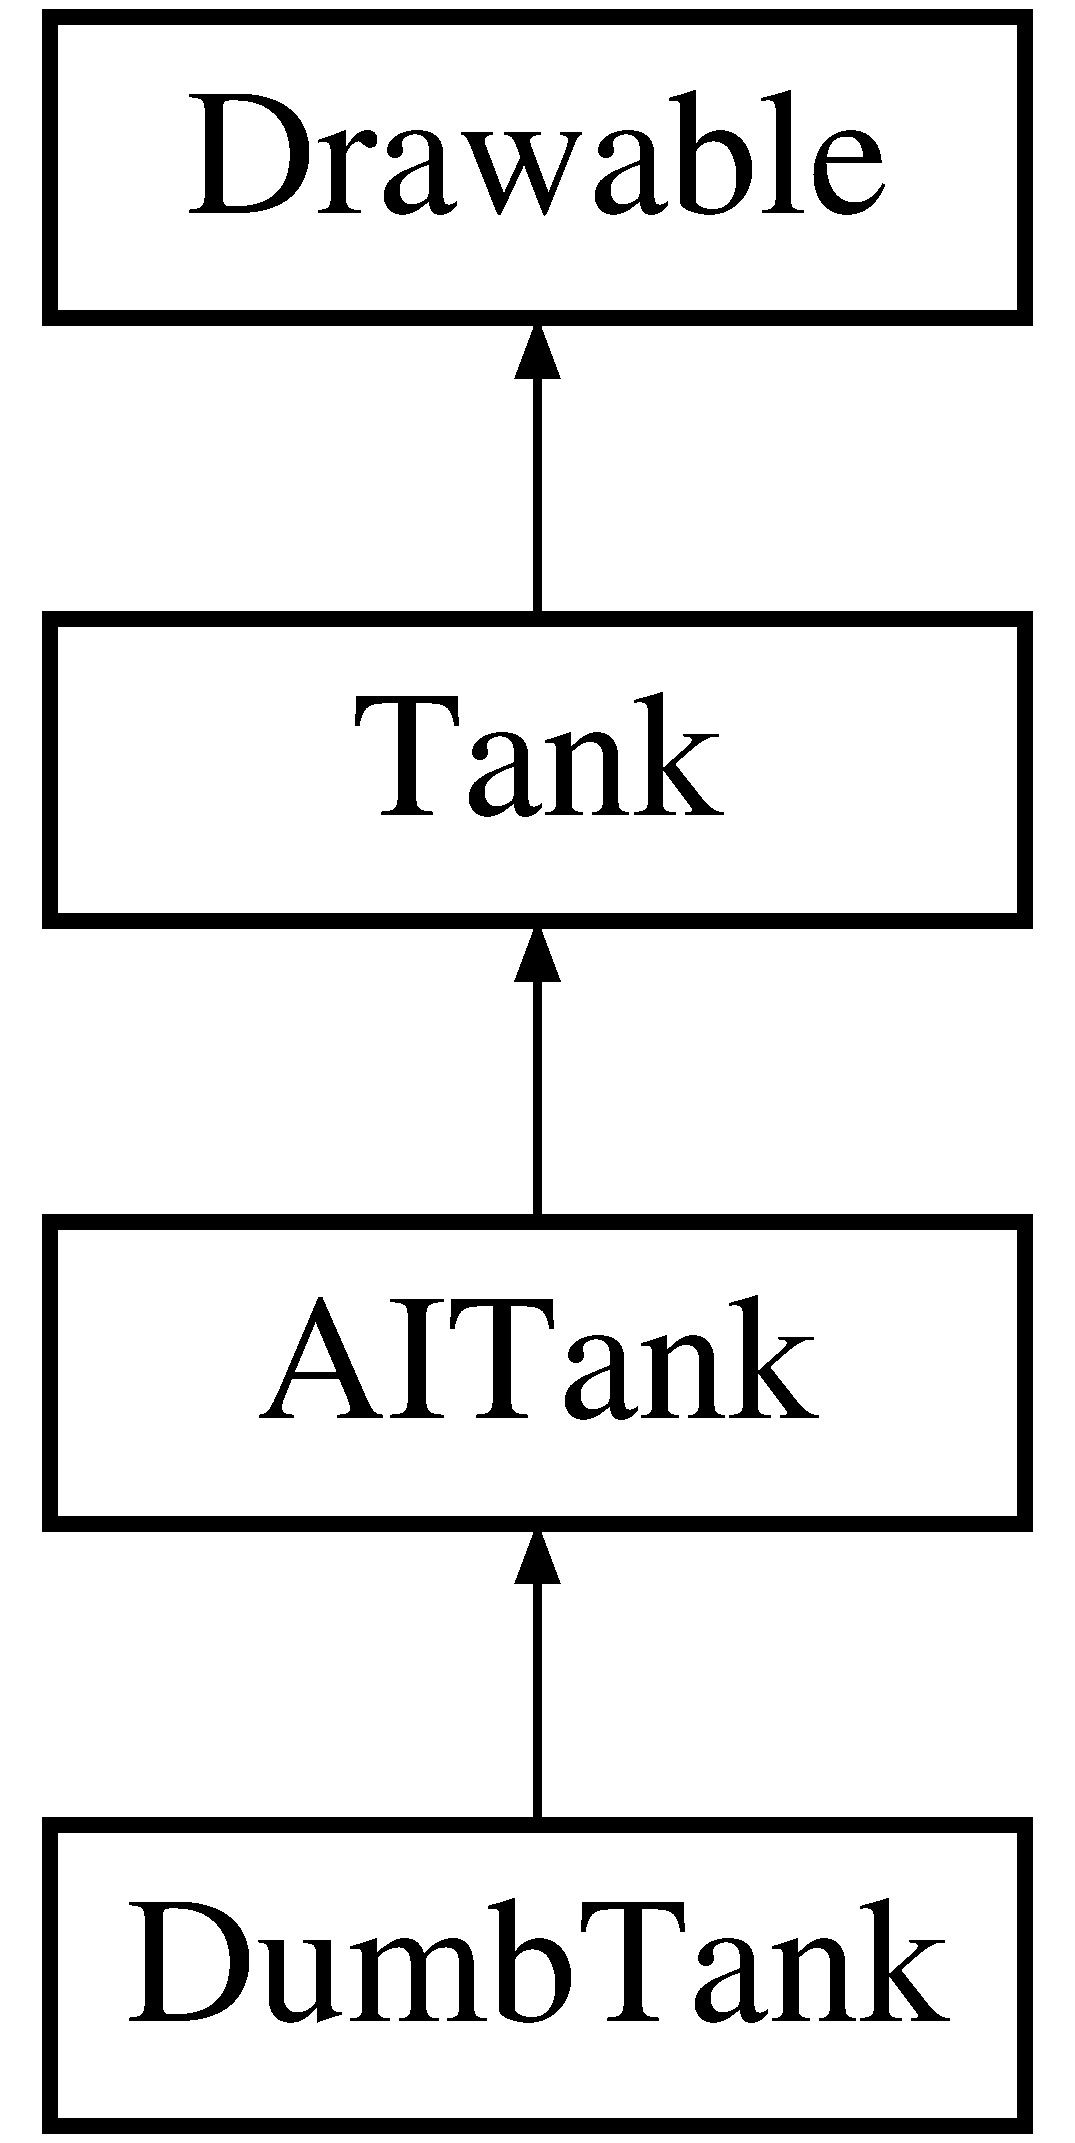
\includegraphics[height=4.000000cm]{class_dumb_tank}
\end{center}
\end{figure}
\subsection*{Public Member Functions}
\begin{DoxyCompactItemize}
\item 
\mbox{\Hypertarget{class_dumb_tank_af30f9ce47648428aa6589cb6e6a0490a}\label{class_dumb_tank_af30f9ce47648428aa6589cb6e6a0490a}} 
void \mbox{\hyperlink{class_dumb_tank_af30f9ce47648428aa6589cb6e6a0490a}{move}} ()
\begin{DoxyCompactList}\small\item\em Move the tank. \end{DoxyCompactList}\item 
\mbox{\Hypertarget{class_dumb_tank_a6d66330ab08b6730a12186ac71d794a0}\label{class_dumb_tank_a6d66330ab08b6730a12186ac71d794a0}} 
void \mbox{\hyperlink{class_dumb_tank_a6d66330ab08b6730a12186ac71d794a0}{reset}} ()
\begin{DoxyCompactList}\small\item\em Reset any variables you need to whent he tank has been shot. \end{DoxyCompactList}\item 
\mbox{\Hypertarget{class_dumb_tank_a2340b3de8f33e3019ab483d56243de5a}\label{class_dumb_tank_a2340b3de8f33e3019ab483d56243de5a}} 
void \mbox{\hyperlink{class_dumb_tank_a2340b3de8f33e3019ab483d56243de5a}{collided}} ()
\begin{DoxyCompactList}\small\item\em Called by the game object when the tank has collided. \end{DoxyCompactList}\item 
\mbox{\Hypertarget{class_dumb_tank_a06dd83683ff628421d6841a8ad8f1877}\label{class_dumb_tank_a06dd83683ff628421d6841a8ad8f1877}} 
void \mbox{\hyperlink{class_dumb_tank_a06dd83683ff628421d6841a8ad8f1877}{mark\+Target}} (\mbox{\hyperlink{class_position}{Position}} p)
\begin{DoxyCompactList}\small\item\em Called by the game object when a target (enemy building) comes within the tanks visible range. \end{DoxyCompactList}\item 
\mbox{\Hypertarget{class_dumb_tank_a6e285a834c2f65bc559c0f08133acc3e}\label{class_dumb_tank_a6e285a834c2f65bc559c0f08133acc3e}} 
void \mbox{\hyperlink{class_dumb_tank_a6e285a834c2f65bc559c0f08133acc3e}{mark\+Enemy}} (\mbox{\hyperlink{class_position}{Position}} p)
\begin{DoxyCompactList}\small\item\em Called by the game object when the enemy tank comes within the tanks visible range. \end{DoxyCompactList}\item 
\mbox{\Hypertarget{class_dumb_tank_ac2c8fe2a13fe009676580b33be241f59}\label{class_dumb_tank_ac2c8fe2a13fe009676580b33be241f59}} 
void \mbox{\hyperlink{class_dumb_tank_ac2c8fe2a13fe009676580b33be241f59}{mark\+Base}} (\mbox{\hyperlink{class_position}{Position}} p)
\begin{DoxyCompactList}\small\item\em Called by the game object when one of you own buildings comes within the tanks visible range. \end{DoxyCompactList}\item 
\mbox{\Hypertarget{class_dumb_tank_a1269c78542b1f504a388aa04fdecc4a8}\label{class_dumb_tank_a1269c78542b1f504a388aa04fdecc4a8}} 
void \mbox{\hyperlink{class_dumb_tank_a1269c78542b1f504a388aa04fdecc4a8}{mark\+Shell}} (\mbox{\hyperlink{class_position}{Position}} p)
\begin{DoxyCompactList}\small\item\em Called by the game object when enemy shell comes within the tanks visible range. \end{DoxyCompactList}\item 
\mbox{\Hypertarget{class_dumb_tank_ad3ee50f39f266ef72106c41d04f7062a}\label{class_dumb_tank_ad3ee50f39f266ef72106c41d04f7062a}} 
bool \mbox{\hyperlink{class_dumb_tank_ad3ee50f39f266ef72106c41d04f7062a}{is\+Firing}} ()
\begin{DoxyCompactList}\small\item\em Called by the game object each frame. When this function returns true (and ammo is availbe and loaded) the tank will fire a shell. \end{DoxyCompactList}\item 
\mbox{\Hypertarget{class_dumb_tank_a5e79dbb66117f72fa22369b4e612cc9a}\label{class_dumb_tank_a5e79dbb66117f72fa22369b4e612cc9a}} 
void {\bfseries score} (int this\+Score, int enemy\+Score)
\end{DoxyCompactItemize}
\subsection*{Additional Inherited Members}


The documentation for this class was generated from the following files\+:\begin{DoxyCompactItemize}
\item 
dumb\+Tank.\+h\item 
dumb\+Tank.\+cpp\end{DoxyCompactItemize}

\hypertarget{class_game}{}\section{Game Class Reference}
\label{class_game}\index{Game@{Game}}
Inheritance diagram for Game\+:\begin{figure}[H]
\begin{center}
\leavevmode
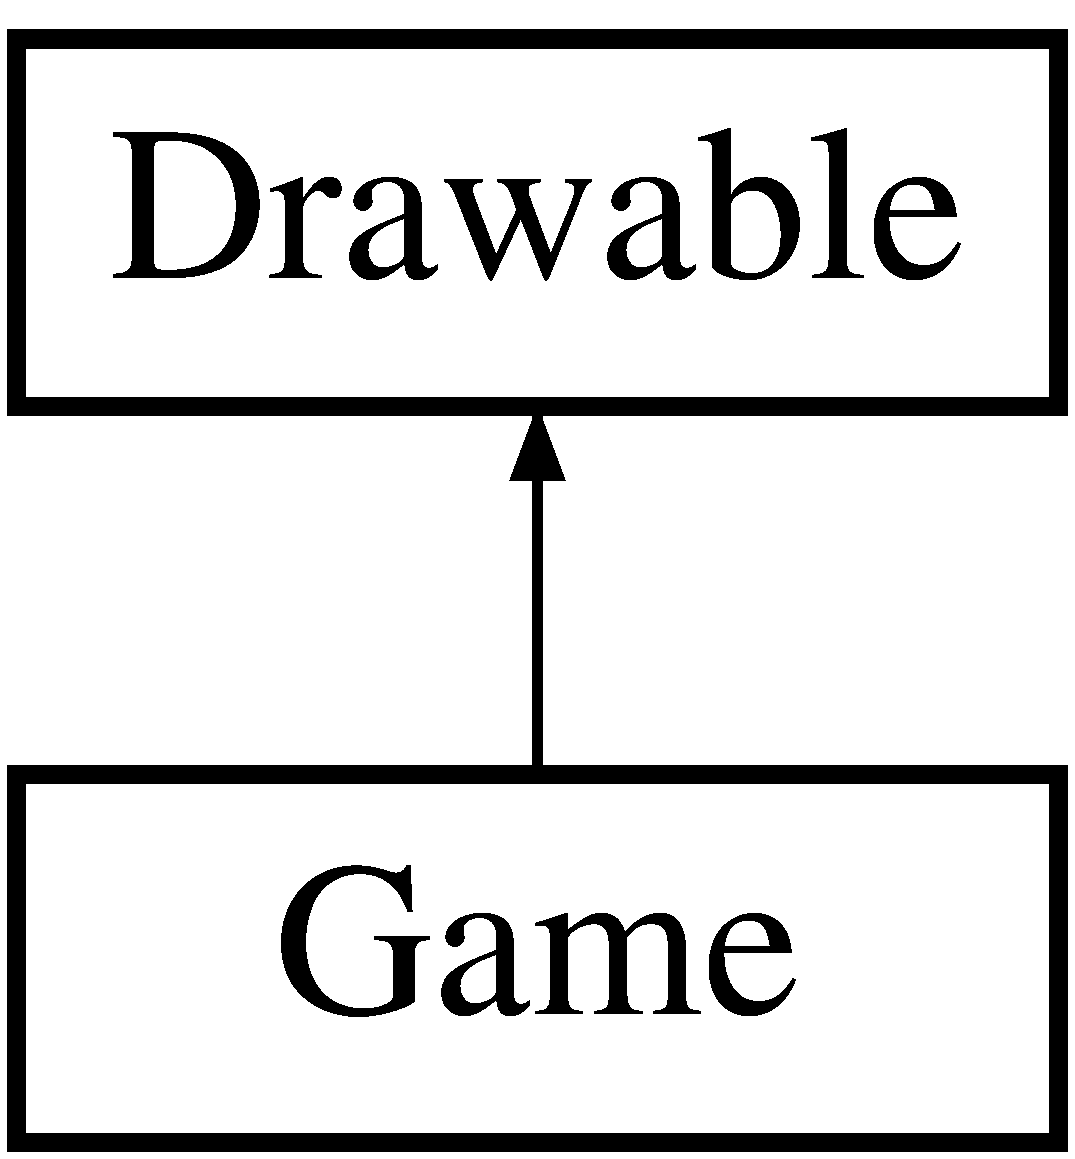
\includegraphics[height=2.000000cm]{class_game}
\end{center}
\end{figure}
\subsection*{Public Member Functions}
\begin{DoxyCompactItemize}
\item 
\mbox{\Hypertarget{class_game_a143d1a2f8a527db60f1fe47ab3d854a7}\label{class_game_a143d1a2f8a527db60f1fe47ab3d854a7}} 
virtual void {\bfseries draw} (sf\+::\+Render\+Target \&target, sf\+::\+Render\+States states) const
\item 
\mbox{\Hypertarget{class_game_aa333825d0bca80e91e53c7e23f053405}\label{class_game_aa333825d0bca80e91e53c7e23f053405}} 
void {\bfseries play} ()
\item 
\mbox{\Hypertarget{class_game_a8bd6da8e86da3a54d5f734ef162955c1}\label{class_game_a8bd6da8e86da3a54d5f734ef162955c1}} 
void {\bfseries key\+Pressed} (sf\+::\+Keyboard\+::\+Key key)
\item 
\mbox{\Hypertarget{class_game_afec9146cc342f8c21a1b23e14da0689a}\label{class_game_afec9146cc342f8c21a1b23e14da0689a}} 
void {\bfseries key\+Released} (sf\+::\+Keyboard\+::\+Key key)
\item 
\mbox{\Hypertarget{class_game_a549cde73db32c59d91f6e7f4fe673d2c}\label{class_game_a549cde73db32c59d91f6e7f4fe673d2c}} 
bool {\bfseries game\+Over} () const
\item 
\mbox{\Hypertarget{class_game_a879cc7faac9e7e5fb2d6caf7fe3ab57b}\label{class_game_a879cc7faac9e7e5fb2d6caf7fe3ab57b}} 
int {\bfseries num\+Blue\+Buildings} () const
\item 
\mbox{\Hypertarget{class_game_a0a33873d2ce5090cbe84840a78eeffc3}\label{class_game_a0a33873d2ce5090cbe84840a78eeffc3}} 
int {\bfseries num\+Red\+Buildings} () const
\end{DoxyCompactItemize}
\subsection*{Public Attributes}
\begin{DoxyCompactItemize}
\item 
\mbox{\Hypertarget{class_game_a96bb9a9bbedbac24f9b230122f663f0c}\label{class_game_a96bb9a9bbedbac24f9b230122f663f0c}} 
\mbox{\hyperlink{class_c_w_tank}{C\+W\+Tank}} {\bfseries npc}
\item 
\mbox{\Hypertarget{class_game_a6b08b37ec5feb1f05188fe86d83615e7}\label{class_game_a6b08b37ec5feb1f05188fe86d83615e7}} 
\mbox{\hyperlink{class_player_tank}{Player\+Tank}} {\bfseries player}
\end{DoxyCompactItemize}


The documentation for this class was generated from the following files\+:\begin{DoxyCompactItemize}
\item 
game.\+h\item 
game.\+cpp\end{DoxyCompactItemize}

\hypertarget{class_obstacle}{}\section{Obstacle Class Reference}
\label{class_obstacle}\index{Obstacle@{Obstacle}}
Inheritance diagram for Obstacle\+:\begin{figure}[H]
\begin{center}
\leavevmode
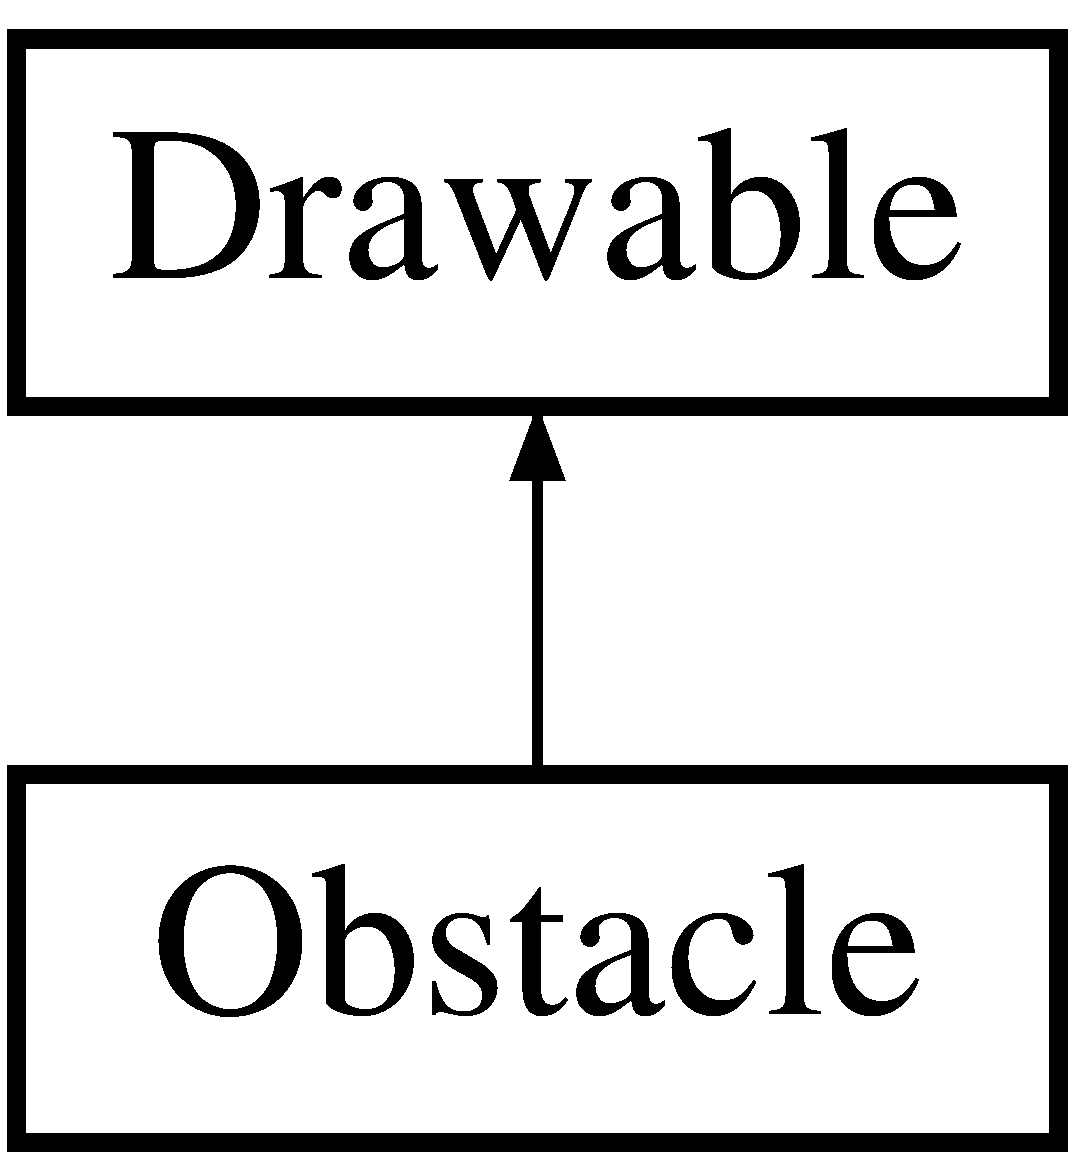
\includegraphics[height=2.000000cm]{class_obstacle}
\end{center}
\end{figure}
\subsection*{Public Member Functions}
\begin{DoxyCompactItemize}
\item 
\mbox{\Hypertarget{class_obstacle_aaded15a33e60984e25e24f0defa50870}\label{class_obstacle_aaded15a33e60984e25e24f0defa50870}} 
{\bfseries Obstacle} (float x1, float y1, float x2, float y2, sf\+::\+Color c)
\item 
\mbox{\Hypertarget{class_obstacle_ab0f2a99b3600ac11ae0247c90f64c071}\label{class_obstacle_ab0f2a99b3600ac11ae0247c90f64c071}} 
virtual void {\bfseries draw} (sf\+::\+Render\+Target \&target, sf\+::\+Render\+States states) const
\item 
\mbox{\Hypertarget{class_obstacle_aa4176e81a3e9d34ebeaf7b44b9080820}\label{class_obstacle_aa4176e81a3e9d34ebeaf7b44b9080820}} 
void {\bfseries set\+Point} (float x, float y)
\item 
\mbox{\Hypertarget{class_obstacle_a3ae1362463a63cd00635013d66f3bcb2}\label{class_obstacle_a3ae1362463a63cd00635013d66f3bcb2}} 
bool {\bfseries operator$<$} (const \mbox{\hyperlink{class_obstacle}{Obstacle}} \&other)
\item 
\mbox{\Hypertarget{class_obstacle_afe9cbf384d3989c1767c04ef9f372ead}\label{class_obstacle_afe9cbf384d3989c1767c04ef9f372ead}} 
void {\bfseries set\+Visible} ()
\item 
\mbox{\Hypertarget{class_obstacle_a81906856ac119daa74363867d81462ad}\label{class_obstacle_a81906856ac119daa74363867d81462ad}} 
bool {\bfseries is\+Visible} () const
\item 
\mbox{\Hypertarget{class_obstacle_ab8ae38eb078cfd5872005e901a02c8af}\label{class_obstacle_ab8ae38eb078cfd5872005e901a02c8af}} 
void {\bfseries toggle\+Debug\+Mode} ()
\end{DoxyCompactItemize}
\subsection*{Public Attributes}
\begin{DoxyCompactItemize}
\item 
\mbox{\Hypertarget{class_obstacle_a65deb910953edc483114ce15d948400e}\label{class_obstacle_a65deb910953edc483114ce15d948400e}} 
\mbox{\hyperlink{class_bounding_box}{Bounding\+Box}} {\bfseries bb}
\item 
\mbox{\Hypertarget{class_obstacle_a7ae604dd6e20ad1a8610dcd38f123c15}\label{class_obstacle_a7ae604dd6e20ad1a8610dcd38f123c15}} 
float {\bfseries dist}
\end{DoxyCompactItemize}


The documentation for this class was generated from the following files\+:\begin{DoxyCompactItemize}
\item 
obstacle.\+h\item 
obstacle.\+cpp\end{DoxyCompactItemize}

\hypertarget{class_player_tank}{}\section{Player\+Tank Class Reference}
\label{class_player_tank}\index{Player\+Tank@{Player\+Tank}}
Inheritance diagram for Player\+Tank\+:\begin{figure}[H]
\begin{center}
\leavevmode
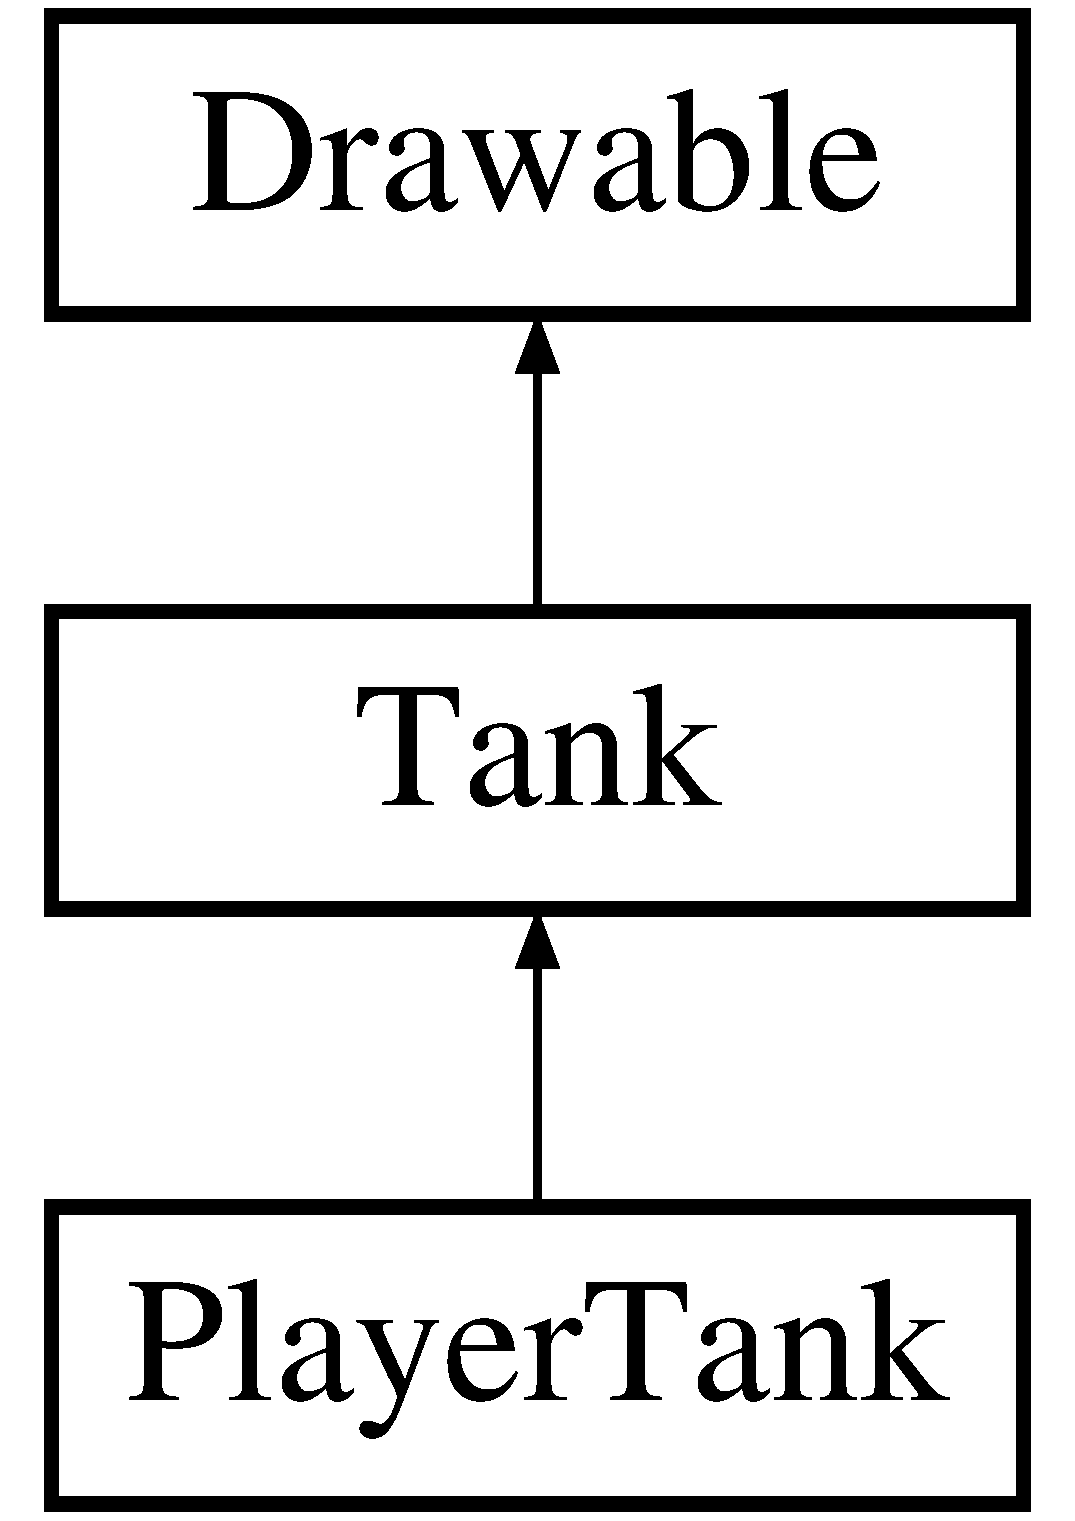
\includegraphics[height=3.000000cm]{class_player_tank}
\end{center}
\end{figure}
\subsection*{Public Member Functions}
\begin{DoxyCompactItemize}
\item 
\mbox{\Hypertarget{class_player_tank_af093b3eb3e479306eff7dd744c733c01}\label{class_player_tank_af093b3eb3e479306eff7dd744c733c01}} 
void {\bfseries move} ()
\item 
\mbox{\Hypertarget{class_player_tank_ab5472bbce0ed243597b93e349889df27}\label{class_player_tank_ab5472bbce0ed243597b93e349889df27}} 
void {\bfseries fire} ()
\item 
\mbox{\Hypertarget{class_player_tank_a0cb62beee428d7b3e61a2670b6bf8f4c}\label{class_player_tank_a0cb62beee428d7b3e61a2670b6bf8f4c}} 
void {\bfseries reset} ()
\end{DoxyCompactItemize}
\subsection*{Additional Inherited Members}


The documentation for this class was generated from the following files\+:\begin{DoxyCompactItemize}
\item 
player\+Tank.\+h\item 
player\+Tank.\+cpp\end{DoxyCompactItemize}

\hypertarget{class_position}{}\section{Position Class Reference}
\label{class_position}\index{Position@{Position}}
\subsection*{Public Member Functions}
\begin{DoxyCompactItemize}
\item 
\mbox{\Hypertarget{class_position_a7890347396c66f6f1eddefce07382abc}\label{class_position_a7890347396c66f6f1eddefce07382abc}} 
{\bfseries Position} (float newX, float newY)
\item 
\mbox{\Hypertarget{class_position_a9c48a9e0efd9db741fd7de5c050b3cc0}\label{class_position_a9c48a9e0efd9db741fd7de5c050b3cc0}} 
void {\bfseries set} (float newX, float newY, float new\+Th)
\item 
\mbox{\Hypertarget{class_position_a252efaf275c7276a6f35338d198de7ee}\label{class_position_a252efaf275c7276a6f35338d198de7ee}} 
float {\bfseries getX} () const
\item 
\mbox{\Hypertarget{class_position_a53ad8ec2f8383db4d615b3fc4e888f77}\label{class_position_a53ad8ec2f8383db4d615b3fc4e888f77}} 
float {\bfseries getY} () const
\item 
\mbox{\Hypertarget{class_position_a2f4eb1b527496eb1175b0545418996e0}\label{class_position_a2f4eb1b527496eb1175b0545418996e0}} 
float {\bfseries get\+Th} () const
\end{DoxyCompactItemize}


The documentation for this class was generated from the following file\+:\begin{DoxyCompactItemize}
\item 
position.\+h\end{DoxyCompactItemize}

\hypertarget{class_shell}{}\section{Shell Class Reference}
\label{class_shell}\index{Shell@{Shell}}
Inheritance diagram for Shell\+:\begin{figure}[H]
\begin{center}
\leavevmode
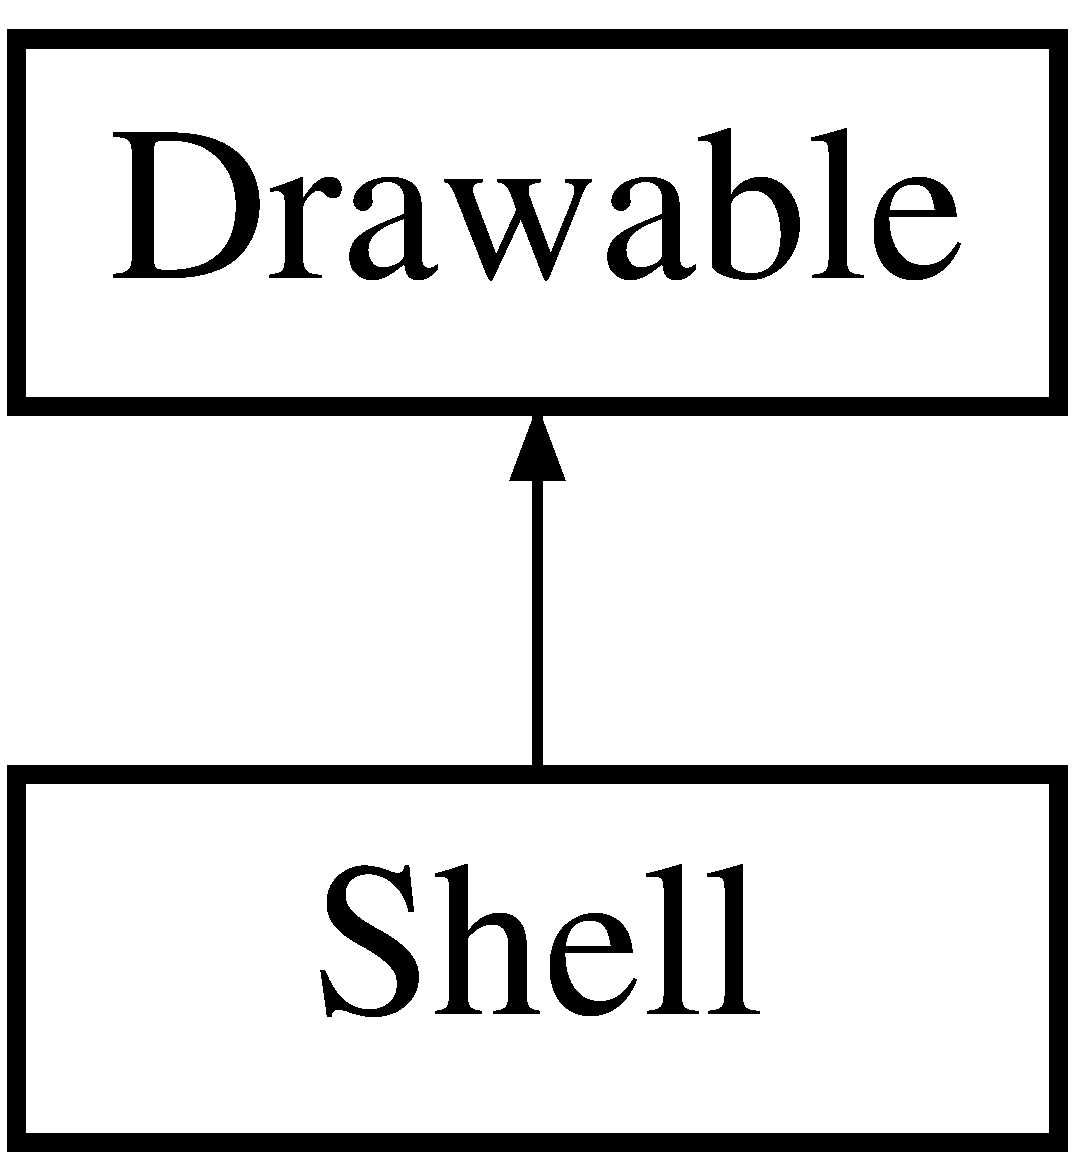
\includegraphics[height=2.000000cm]{class_shell}
\end{center}
\end{figure}
\subsection*{Public Member Functions}
\begin{DoxyCompactItemize}
\item 
\mbox{\Hypertarget{class_shell_aa393a4a63b6217e3ee9d03cf65564d07}\label{class_shell_aa393a4a63b6217e3ee9d03cf65564d07}} 
{\bfseries Shell} (\mbox{\hyperlink{class_position}{Position}} pos, bool is\+N\+PC)
\item 
\mbox{\Hypertarget{class_shell_a9520ac56a223315a10ed177dae067fc5}\label{class_shell_a9520ac56a223315a10ed177dae067fc5}} 
virtual void {\bfseries draw} (sf\+::\+Render\+Target \&target, sf\+::\+Render\+States states) const
\item 
\mbox{\Hypertarget{class_shell_a4cf835ccfa6212c713c428777f98f8fc}\label{class_shell_a4cf835ccfa6212c713c428777f98f8fc}} 
void {\bfseries move} ()
\item 
\mbox{\Hypertarget{class_shell_a0d5a59882864dd32f5e4c8f9a958e435}\label{class_shell_a0d5a59882864dd32f5e4c8f9a958e435}} 
float {\bfseries getX} ()
\item 
\mbox{\Hypertarget{class_shell_a69b65e13952ea6784e2d5155a5f92a7d}\label{class_shell_a69b65e13952ea6784e2d5155a5f92a7d}} 
float {\bfseries getY} ()
\item 
\mbox{\Hypertarget{class_shell_a43e70755fa534909ab2d6a75d7e485c8}\label{class_shell_a43e70755fa534909ab2d6a75d7e485c8}} 
void {\bfseries toggle\+Debug\+Mode} ()
\item 
\mbox{\Hypertarget{class_shell_aef07642873e5d37247d3a0e81f892173}\label{class_shell_aef07642873e5d37247d3a0e81f892173}} 
void {\bfseries set\+Visible} ()
\item 
\mbox{\Hypertarget{class_shell_a0801948fa62e656bef93e75f722d456f}\label{class_shell_a0801948fa62e656bef93e75f722d456f}} 
bool {\bfseries is\+Visible} () const
\item 
\mbox{\Hypertarget{class_shell_a3e949dd122d6db50fb23ddceb1e3a1ef}\label{class_shell_a3e949dd122d6db50fb23ddceb1e3a1ef}} 
bool {\bfseries is\+Npc} () const
\item 
\mbox{\Hypertarget{class_shell_a4e536448e437dff85ed7911ef6cfd854}\label{class_shell_a4e536448e437dff85ed7911ef6cfd854}} 
bool {\bfseries could\+See\+When\+Fired} (\mbox{\hyperlink{class_bounding_box}{Bounding\+Box}} object)
\end{DoxyCompactItemize}
\subsection*{Public Attributes}
\begin{DoxyCompactItemize}
\item 
\mbox{\Hypertarget{class_shell_a111217ec1fa16f95690a68a6f3150048}\label{class_shell_a111217ec1fa16f95690a68a6f3150048}} 
\mbox{\hyperlink{class_bounding_box}{Bounding\+Box}} {\bfseries bb}
\end{DoxyCompactItemize}
\subsection*{Protected Member Functions}
\begin{DoxyCompactItemize}
\item 
\mbox{\Hypertarget{class_shell_a59fee1db1f35166986121dfcdbab3a4f}\label{class_shell_a59fee1db1f35166986121dfcdbab3a4f}} 
void {\bfseries update\+Bb} ()
\end{DoxyCompactItemize}
\subsection*{Protected Attributes}
\begin{DoxyCompactItemize}
\item 
\mbox{\Hypertarget{class_shell_aa616cb1bfcd1e807c1bcaeef8fea691e}\label{class_shell_aa616cb1bfcd1e807c1bcaeef8fea691e}} 
\mbox{\hyperlink{class_position}{Position}} {\bfseries pos}
\item 
\mbox{\Hypertarget{class_shell_a3767a511c51267156173ee866a3328b7}\label{class_shell_a3767a511c51267156173ee866a3328b7}} 
\mbox{\hyperlink{class_position}{Position}} {\bfseries firing\+Position}
\item 
\mbox{\Hypertarget{class_shell_a79b3bf24805872c786092a3ac9269707}\label{class_shell_a79b3bf24805872c786092a3ac9269707}} 
sf\+::\+Rectangle\+Shape {\bfseries box}
\item 
\mbox{\Hypertarget{class_shell_a08fbc870060f59807f45e5ee08841151}\label{class_shell_a08fbc870060f59807f45e5ee08841151}} 
bool {\bfseries debug\+Mode}
\item 
\mbox{\Hypertarget{class_shell_ac61119f0a9d9941ae0d66c12d124e2e6}\label{class_shell_ac61119f0a9d9941ae0d66c12d124e2e6}} 
bool {\bfseries visible}
\item 
\mbox{\Hypertarget{class_shell_a33a31cb9ce411ec7eed0a3a8105f8a35}\label{class_shell_a33a31cb9ce411ec7eed0a3a8105f8a35}} 
bool {\bfseries npc}
\end{DoxyCompactItemize}


The documentation for this class was generated from the following files\+:\begin{DoxyCompactItemize}
\item 
shell.\+h\item 
shell.\+cpp\end{DoxyCompactItemize}

\hypertarget{class_tank}{}\section{Tank Class Reference}
\label{class_tank}\index{Tank@{Tank}}
Inheritance diagram for Tank\+:\begin{figure}[H]
\begin{center}
\leavevmode
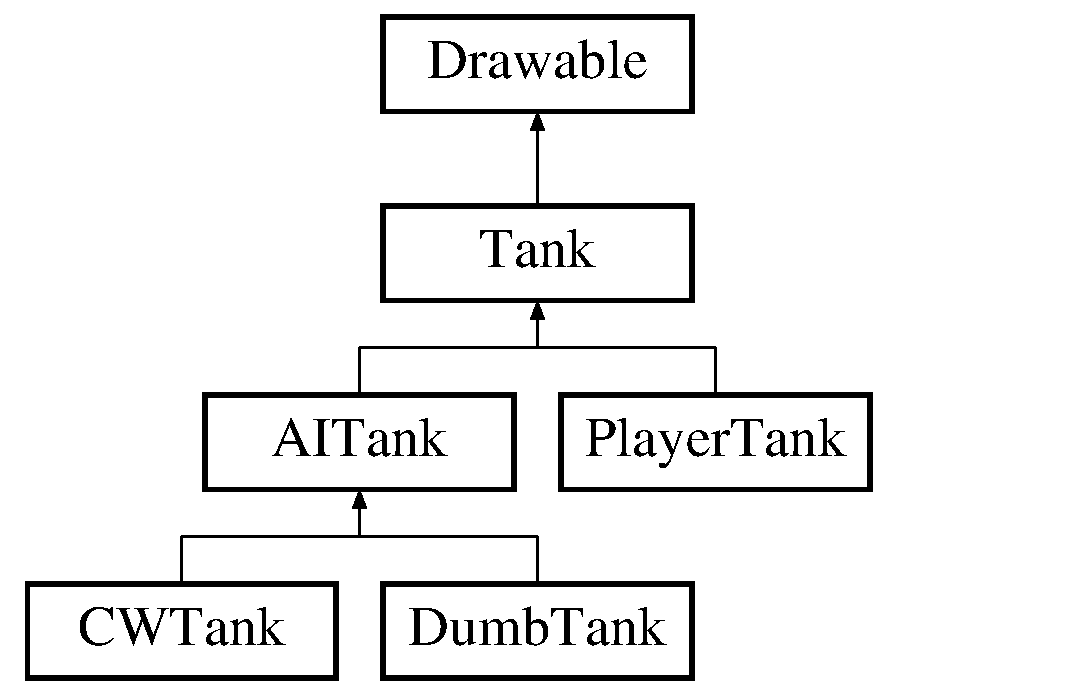
\includegraphics[height=4.000000cm]{class_tank}
\end{center}
\end{figure}
\subsection*{Public Member Functions}
\begin{DoxyCompactItemize}
\item 
\mbox{\Hypertarget{class_tank_a83ff27f2cff5926c8c970751084af8f7}\label{class_tank_a83ff27f2cff5926c8c970751084af8f7}} 
virtual void \mbox{\hyperlink{class_tank_a83ff27f2cff5926c8c970751084af8f7}{draw}} (sf\+::\+Render\+Target \&target, sf\+::\+Render\+States states) const
\begin{DoxyCompactList}\small\item\em Draw \mbox{\hyperlink{class_tank}{Tank}}. \end{DoxyCompactList}\item 
\mbox{\Hypertarget{class_tank_a2cf1b4e5397bf54df4906e8c3f91a554}\label{class_tank_a2cf1b4e5397bf54df4906e8c3f91a554}} 
void \mbox{\hyperlink{class_tank_a2cf1b4e5397bf54df4906e8c3f91a554}{reset\+Tank}} (float newX, float newY, float new\+Th, float new\+Turret\+Th)
\begin{DoxyCompactList}\small\item\em Reset \mbox{\hyperlink{class_tank}{Tank}}\textquotesingle{}s position. \end{DoxyCompactList}\item 
\mbox{\Hypertarget{class_tank_a12273b8cb5c553dbe2d86ee1901e7724}\label{class_tank_a12273b8cb5c553dbe2d86ee1901e7724}} 
void \mbox{\hyperlink{class_tank_a12273b8cb5c553dbe2d86ee1901e7724}{go\+Forward}} ()
\begin{DoxyCompactList}\small\item\em Set the tank to go forwards. \end{DoxyCompactList}\item 
\mbox{\Hypertarget{class_tank_aa051fc7515586360ab4f92f48a0ac320}\label{class_tank_aa051fc7515586360ab4f92f48a0ac320}} 
void \mbox{\hyperlink{class_tank_aa051fc7515586360ab4f92f48a0ac320}{go\+Backward}} ()
\begin{DoxyCompactList}\small\item\em Set the tank to go backwards. \end{DoxyCompactList}\item 
\mbox{\Hypertarget{class_tank_a216e88194fedd737d9382e31adbe032c}\label{class_tank_a216e88194fedd737d9382e31adbe032c}} 
void \mbox{\hyperlink{class_tank_a216e88194fedd737d9382e31adbe032c}{go\+Left}} ()
\begin{DoxyCompactList}\small\item\em Set the tank to go left. \end{DoxyCompactList}\item 
\mbox{\Hypertarget{class_tank_a18f5109098cccf51b7a3c1b6ac78f0ef}\label{class_tank_a18f5109098cccf51b7a3c1b6ac78f0ef}} 
void \mbox{\hyperlink{class_tank_a18f5109098cccf51b7a3c1b6ac78f0ef}{go\+Right}} ()
\begin{DoxyCompactList}\small\item\em Set the tank to go right. \end{DoxyCompactList}\item 
\mbox{\Hypertarget{class_tank_a576e0c46b45fdfa6e9bf070d2861488a}\label{class_tank_a576e0c46b45fdfa6e9bf070d2861488a}} 
void \mbox{\hyperlink{class_tank_a576e0c46b45fdfa6e9bf070d2861488a}{turret\+Go\+Left}} ()
\begin{DoxyCompactList}\small\item\em Set the turret to go left. \end{DoxyCompactList}\item 
\mbox{\Hypertarget{class_tank_a24db99775a2b58a7d476712b0f37b492}\label{class_tank_a24db99775a2b58a7d476712b0f37b492}} 
void \mbox{\hyperlink{class_tank_a24db99775a2b58a7d476712b0f37b492}{turret\+Go\+Right}} ()
\begin{DoxyCompactList}\small\item\em Set the turret to go right. \end{DoxyCompactList}\item 
\mbox{\Hypertarget{class_tank_a1784370e1c19b26fb5072496ce7d8e8f}\label{class_tank_a1784370e1c19b26fb5072496ce7d8e8f}} 
void \mbox{\hyperlink{class_tank_a1784370e1c19b26fb5072496ce7d8e8f}{stop}} ()
\begin{DoxyCompactList}\small\item\em Stop the tank body movement. \end{DoxyCompactList}\item 
\mbox{\Hypertarget{class_tank_accc892bf77ffe29acf3a480ebe783c25}\label{class_tank_accc892bf77ffe29acf3a480ebe783c25}} 
void \mbox{\hyperlink{class_tank_accc892bf77ffe29acf3a480ebe783c25}{stop\+Turret}} ()
\begin{DoxyCompactList}\small\item\em Stop the turret movement. \end{DoxyCompactList}\item 
\mbox{\Hypertarget{class_tank_ab908518b154816de8a5dfa0b3450ca3f}\label{class_tank_ab908518b154816de8a5dfa0b3450ca3f}} 
void \mbox{\hyperlink{class_tank_ab908518b154816de8a5dfa0b3450ca3f}{mark\+Pos}} ()
\begin{DoxyCompactList}\small\item\em Record the prevoius position. \end{DoxyCompactList}\item 
\mbox{\Hypertarget{class_tank_a656fff479053496146ac731b851e38ac}\label{class_tank_a656fff479053496146ac731b851e38ac}} 
void \mbox{\hyperlink{class_tank_a656fff479053496146ac731b851e38ac}{recall\+Pos}} ()
\begin{DoxyCompactList}\small\item\em Go back to the prevoius position -\/ simple form of position correction. \end{DoxyCompactList}\item 
\mbox{\Hypertarget{class_tank_a381debea1a8951fa633051343565a76b}\label{class_tank_a381debea1a8951fa633051343565a76b}} 
void \mbox{\hyperlink{class_tank_a381debea1a8951fa633051343565a76b}{fire\+Shell}} ()
\begin{DoxyCompactList}\small\item\em Fire a shell. \end{DoxyCompactList}\item 
\mbox{\Hypertarget{class_tank_ae7bb118a1220a1f0a3cce20017499bd8}\label{class_tank_ae7bb118a1220a1f0a3cce20017499bd8}} 
virtual void {\bfseries move} ()=0
\item 
\mbox{\Hypertarget{class_tank_a251760fd6484b08389e70712387e42b1}\label{class_tank_a251760fd6484b08389e70712387e42b1}} 
void \mbox{\hyperlink{class_tank_a251760fd6484b08389e70712387e42b1}{implement\+Move}} ()
\begin{DoxyCompactList}\small\item\em Move tank, relise what is in the move funtion. \end{DoxyCompactList}\item 
\mbox{\Hypertarget{class_tank_a5a801ccb0e922bf03b46da1d6e07c49f}\label{class_tank_a5a801ccb0e922bf03b46da1d6e07c49f}} 
\mbox{\hyperlink{class_position}{Position}} \mbox{\hyperlink{class_tank_a5a801ccb0e922bf03b46da1d6e07c49f}{firing\+Position}} () const
\begin{DoxyCompactList}\small\item\em \mbox{\hyperlink{class_position}{Position}} of the tank as shell is fired. \end{DoxyCompactList}\item 
\mbox{\Hypertarget{class_tank_aeab5ff8d3aff0512111c7efded049f89}\label{class_tank_aeab5ff8d3aff0512111c7efded049f89}} 
float \mbox{\hyperlink{class_tank_aeab5ff8d3aff0512111c7efded049f89}{getX}} () const
\begin{DoxyCompactList}\small\item\em \mbox{\hyperlink{class_position}{Position}} of the tank in x. \end{DoxyCompactList}\item 
\mbox{\Hypertarget{class_tank_a77c97bf9da4ec98e0659541dfa5305f5}\label{class_tank_a77c97bf9da4ec98e0659541dfa5305f5}} 
float \mbox{\hyperlink{class_tank_a77c97bf9da4ec98e0659541dfa5305f5}{getY}} () const
\begin{DoxyCompactList}\small\item\em \mbox{\hyperlink{class_position}{Position}} of the tank in y. \end{DoxyCompactList}\item 
\mbox{\Hypertarget{class_tank_af43b411fce8177c0206fdabb9fd68f51}\label{class_tank_af43b411fce8177c0206fdabb9fd68f51}} 
int \mbox{\hyperlink{class_tank_af43b411fce8177c0206fdabb9fd68f51}{get\+Number\+Of\+Shells}} () const
\begin{DoxyCompactList}\small\item\em Amount of ammo left. \end{DoxyCompactList}\item 
\mbox{\Hypertarget{class_tank_a597b2c051340cce63e7b5bcb6fa5c39c}\label{class_tank_a597b2c051340cce63e7b5bcb6fa5c39c}} 
bool \mbox{\hyperlink{class_tank_a597b2c051340cce63e7b5bcb6fa5c39c}{can\+See}} (\mbox{\hyperlink{class_bounding_box}{Bounding\+Box}} other) const
\begin{DoxyCompactList}\small\item\em Can this tank see the bounding box? \end{DoxyCompactList}\item 
\mbox{\Hypertarget{class_tank_a6a39f37aa7ebbf66d0661815c43b37ef}\label{class_tank_a6a39f37aa7ebbf66d0661815c43b37ef}} 
bool \mbox{\hyperlink{class_tank_a6a39f37aa7ebbf66d0661815c43b37ef}{can\+Fire}} () const
\begin{DoxyCompactList}\small\item\em Can this tnak fire. \end{DoxyCompactList}\item 
\mbox{\Hypertarget{class_tank_a584ef5a0ec4095ca9407fb853677c7f0}\label{class_tank_a584ef5a0ec4095ca9407fb853677c7f0}} 
bool \mbox{\hyperlink{class_tank_a584ef5a0ec4095ca9407fb853677c7f0}{has\+Ammo}} () const
\begin{DoxyCompactList}\small\item\em Does this tank have nay ammo left. \end{DoxyCompactList}\item 
\mbox{\Hypertarget{class_tank_a4126dc18c8684e126ba01b45bebc6b62}\label{class_tank_a4126dc18c8684e126ba01b45bebc6b62}} 
void \mbox{\hyperlink{class_tank_a4126dc18c8684e126ba01b45bebc6b62}{toggle\+Debug\+Mode}} ()
\begin{DoxyCompactList}\small\item\em Toggle the debug mode. \end{DoxyCompactList}\end{DoxyCompactItemize}
\subsection*{Public Attributes}
\begin{DoxyCompactItemize}
\item 
\mbox{\Hypertarget{class_tank_a8ceaceb9194a65d896947290a9394d8e}\label{class_tank_a8ceaceb9194a65d896947290a9394d8e}} 
\mbox{\hyperlink{class_bounding_box}{Bounding\+Box}} \mbox{\hyperlink{class_tank_a8ceaceb9194a65d896947290a9394d8e}{bb}}
\begin{DoxyCompactList}\small\item\em BB for collision detection. \end{DoxyCompactList}\end{DoxyCompactItemize}
\subsection*{Protected Member Functions}
\begin{DoxyCompactItemize}
\item 
\mbox{\Hypertarget{class_tank_ad6df73f502e84c0e96c67f8d53671373}\label{class_tank_ad6df73f502e84c0e96c67f8d53671373}} 
void \mbox{\hyperlink{class_tank_ad6df73f502e84c0e96c67f8d53671373}{clear\+Movement}} ()
\begin{DoxyCompactList}\small\item\em Stop current movement. \end{DoxyCompactList}\item 
\mbox{\Hypertarget{class_tank_a893c47a8494ea5a01edf8cc96e0932a6}\label{class_tank_a893c47a8494ea5a01edf8cc96e0932a6}} 
void \mbox{\hyperlink{class_tank_a893c47a8494ea5a01edf8cc96e0932a6}{update\+Bb}} ()
\begin{DoxyCompactList}\small\item\em Update the bounding box position to be the same as the tank. \end{DoxyCompactList}\end{DoxyCompactItemize}
\subsection*{Protected Attributes}
\begin{DoxyCompactItemize}
\item 
\mbox{\Hypertarget{class_tank_ab74eb809bf4c7855b01796b2f1eec1b1}\label{class_tank_ab74eb809bf4c7855b01796b2f1eec1b1}} 
\mbox{\hyperlink{class_position}{Position}} \mbox{\hyperlink{class_tank_ab74eb809bf4c7855b01796b2f1eec1b1}{pos}}
\begin{DoxyCompactList}\small\item\em Current position of the tank. \end{DoxyCompactList}\item 
\mbox{\Hypertarget{class_tank_a786298cf02e081b0c8bc7598c8f6a68d}\label{class_tank_a786298cf02e081b0c8bc7598c8f6a68d}} 
\mbox{\hyperlink{class_position}{Position}} \mbox{\hyperlink{class_tank_a786298cf02e081b0c8bc7598c8f6a68d}{old\+Pos}}
\begin{DoxyCompactList}\small\item\em Previous position of the tank, used in very basic position correction for collisions. \end{DoxyCompactList}\item 
\mbox{\Hypertarget{class_tank_ac0a54abd647f79b9087efccce9188014}\label{class_tank_ac0a54abd647f79b9087efccce9188014}} 
float \mbox{\hyperlink{class_tank_ac0a54abd647f79b9087efccce9188014}{turret\+Th}}
\begin{DoxyCompactList}\small\item\em Current heading of the gun turret. \end{DoxyCompactList}\item 
\mbox{\Hypertarget{class_tank_ab1b1e42e323c8e52276857887cb624f0}\label{class_tank_ab1b1e42e323c8e52276857887cb624f0}} 
int \mbox{\hyperlink{class_tank_ab1b1e42e323c8e52276857887cb624f0}{number\+Of\+Shells}}
\begin{DoxyCompactList}\small\item\em Amount of ammo left. \end{DoxyCompactList}\item 
\mbox{\Hypertarget{class_tank_a83bd2e7cd94cb7325f16e443a4a39d8e}\label{class_tank_a83bd2e7cd94cb7325f16e443a4a39d8e}} 
bool \mbox{\hyperlink{class_tank_a83bd2e7cd94cb7325f16e443a4a39d8e}{forward}}
\begin{DoxyCompactList}\small\item\em \mbox{\hyperlink{class_tank}{Tank}} moving forwards. \end{DoxyCompactList}\item 
\mbox{\Hypertarget{class_tank_a8d2b0d753ca8a7e2462b6a3e53bcf450}\label{class_tank_a8d2b0d753ca8a7e2462b6a3e53bcf450}} 
bool \mbox{\hyperlink{class_tank_a8d2b0d753ca8a7e2462b6a3e53bcf450}{backward}}
\begin{DoxyCompactList}\small\item\em \mbox{\hyperlink{class_tank}{Tank}} moving backwards. \end{DoxyCompactList}\item 
\mbox{\Hypertarget{class_tank_a6bca5d0c431fb2ecc7ca2f9b34b5e99b}\label{class_tank_a6bca5d0c431fb2ecc7ca2f9b34b5e99b}} 
bool \mbox{\hyperlink{class_tank_a6bca5d0c431fb2ecc7ca2f9b34b5e99b}{left}}
\begin{DoxyCompactList}\small\item\em \mbox{\hyperlink{class_tank}{Tank}} turning left. \end{DoxyCompactList}\item 
\mbox{\Hypertarget{class_tank_ad12b6cf70d0cd85bc574ec5059d3d925}\label{class_tank_ad12b6cf70d0cd85bc574ec5059d3d925}} 
bool \mbox{\hyperlink{class_tank_ad12b6cf70d0cd85bc574ec5059d3d925}{right}}
\begin{DoxyCompactList}\small\item\em Tnak turning right. \end{DoxyCompactList}\item 
\mbox{\Hypertarget{class_tank_abc5be1fb4ae64b5ea39bffd6f11e2a65}\label{class_tank_abc5be1fb4ae64b5ea39bffd6f11e2a65}} 
bool \mbox{\hyperlink{class_tank_abc5be1fb4ae64b5ea39bffd6f11e2a65}{turret\+Left}}
\begin{DoxyCompactList}\small\item\em Turret turning left. \end{DoxyCompactList}\item 
\mbox{\Hypertarget{class_tank_a095e8e9592ca8c33030ae9d15f28aea8}\label{class_tank_a095e8e9592ca8c33030ae9d15f28aea8}} 
bool \mbox{\hyperlink{class_tank_a095e8e9592ca8c33030ae9d15f28aea8}{turret\+Right}}
\begin{DoxyCompactList}\small\item\em Turret turing right. \end{DoxyCompactList}\item 
\mbox{\Hypertarget{class_tank_a923e760c9a624f97511d8be33226532f}\label{class_tank_a923e760c9a624f97511d8be33226532f}} 
sf\+::\+Sprite \mbox{\hyperlink{class_tank_a923e760c9a624f97511d8be33226532f}{body}}
\begin{DoxyCompactList}\small\item\em Sprite used to draw the tank. \end{DoxyCompactList}\item 
\mbox{\Hypertarget{class_tank_a817b1646c30f381340304fcd4b88fb3e}\label{class_tank_a817b1646c30f381340304fcd4b88fb3e}} 
sf\+::\+Texture \mbox{\hyperlink{class_tank_a817b1646c30f381340304fcd4b88fb3e}{body\+Tex}}
\begin{DoxyCompactList}\small\item\em Texture used by the tank sprite. \end{DoxyCompactList}\item 
\mbox{\Hypertarget{class_tank_af180aa607b98adf48c8064b1c78f14e3}\label{class_tank_af180aa607b98adf48c8064b1c78f14e3}} 
sf\+::\+Sprite \mbox{\hyperlink{class_tank_af180aa607b98adf48c8064b1c78f14e3}{turret}}
\begin{DoxyCompactList}\small\item\em Sprite used to draw the tanks turret. \end{DoxyCompactList}\item 
\mbox{\Hypertarget{class_tank_a60849721eb299a75ceaacbde0565fe97}\label{class_tank_a60849721eb299a75ceaacbde0565fe97}} 
sf\+::\+Texture \mbox{\hyperlink{class_tank_a60849721eb299a75ceaacbde0565fe97}{turret\+Tex}}
\begin{DoxyCompactList}\small\item\em Texture used by the tank turret sprite. \end{DoxyCompactList}\item 
\mbox{\Hypertarget{class_tank_a891f14d486b465194b9cd043b07451ba}\label{class_tank_a891f14d486b465194b9cd043b07451ba}} 
bool \mbox{\hyperlink{class_tank_a891f14d486b465194b9cd043b07451ba}{debug\+Mode}}
\begin{DoxyCompactList}\small\item\em Debug mode -\/ show more stuff. \end{DoxyCompactList}\end{DoxyCompactItemize}


The documentation for this class was generated from the following files\+:\begin{DoxyCompactItemize}
\item 
tank.\+h\item 
tank.\+cpp\end{DoxyCompactItemize}

%--- End generated contents ---

% Index
\backmatter
\newpage
\phantomsection
\clearemptydoublepage
\addcontentsline{toc}{chapter}{Index}
\printindex

\end{document}
